\chapter{Design Overview}

This chapter will include the old Building Block and Runtime View. 

This chapter is going to describe the static decomposition of the system into building blocks. It is going to show also the relationship between these blocks.
This chapter describes the behavior and interaction of the system’s building blocks as runtime elements.

\section{Overview}
\begin{figure}[htp]
\centering
	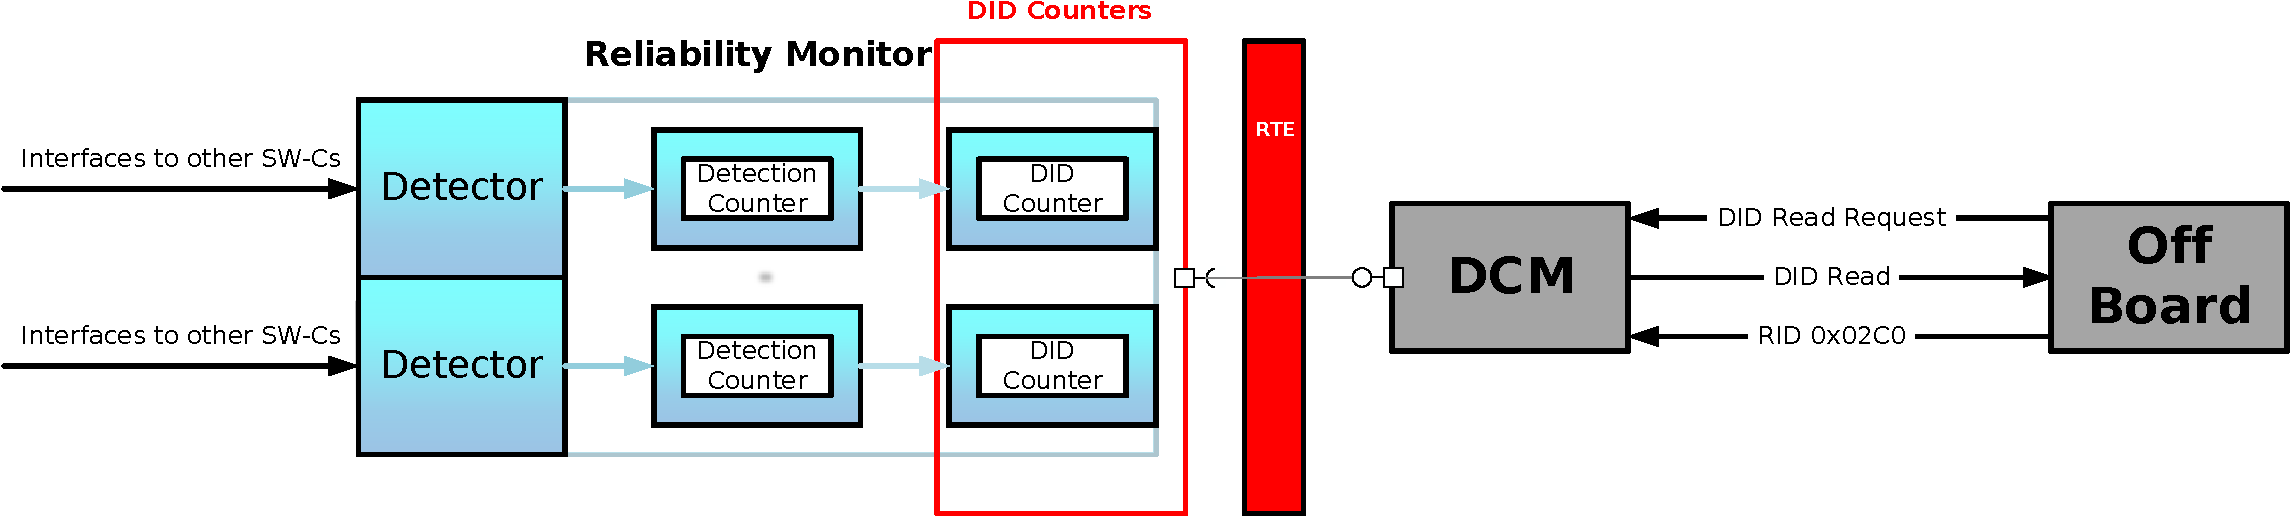
\includegraphics[width=\textwidth]{images/Monitors}
	\caption{Example reliability monitor detectors, DID counters, DID read or RID execution}
	\label{fig:Monitors}
\end{figure}

The SUM_SOH is defined to deploy functionalities needed to support monitoring and reporting of multiple facets of the operational health of the host ECU communication systems, hardware, operating system and software components.

The SUM\_SOH design requires the use of software design elements called reliability monitors and detectors to support the implementation of infrastructure related functions (Figure~\ref{fig:Monitors}).

The SUM\_SOH reliability monitors are software functions that rely on one or more logically grouped internal and/or \textbf{external} detectors to filter and record the performance metrics of similar operating system constructs such as memory operation, network communication behavior and reset behavior (Figure~\ref{fig:Block_view}).

The SUM\_SOH detectors are software functions defined in \textbf{software performance specifications}. They are used for monitoring the performance of supervised/monitored operations, but can also be useful for functionalities other than those associated with reliability monitors.

The SUM_SOH requirements define detection counters used to maintain the raw count of specific errors or faults recorded by detectors.

Filtering of events based on defined calibration values is required for the SUM_SOH implementation, and to that end the requirements define multiple DID counters needed to maintain the filtered count of specific events.

Moreover, the SUM\_SOH provides data regarding monitored events via DIDs allocated for the SUM\_SOH and SUM\_ERRH.

The SUM_SOH detectors can use one of two types of filtering:
\begin{itemize}
	\item Threshold filtering. This type of filtering defines a threshold on the count of monitored events as a calibration value to be used by the SUM_SOH. Once the defined threshold is reached the SUM_SOH will take the following actions.  
	\item Threshold during a time window filtering. In this type of filtering, two calibration values are defined to be used by the SUM_SOH. The first is a threshold of the detection count of monitored events and the second is a threshold of the events detection time window. If the threshold of events is reached within the defined time window threshold, the SUM_SOH will take the following actions.
\end{itemize}

\begin{figure}[htp]
\centering
	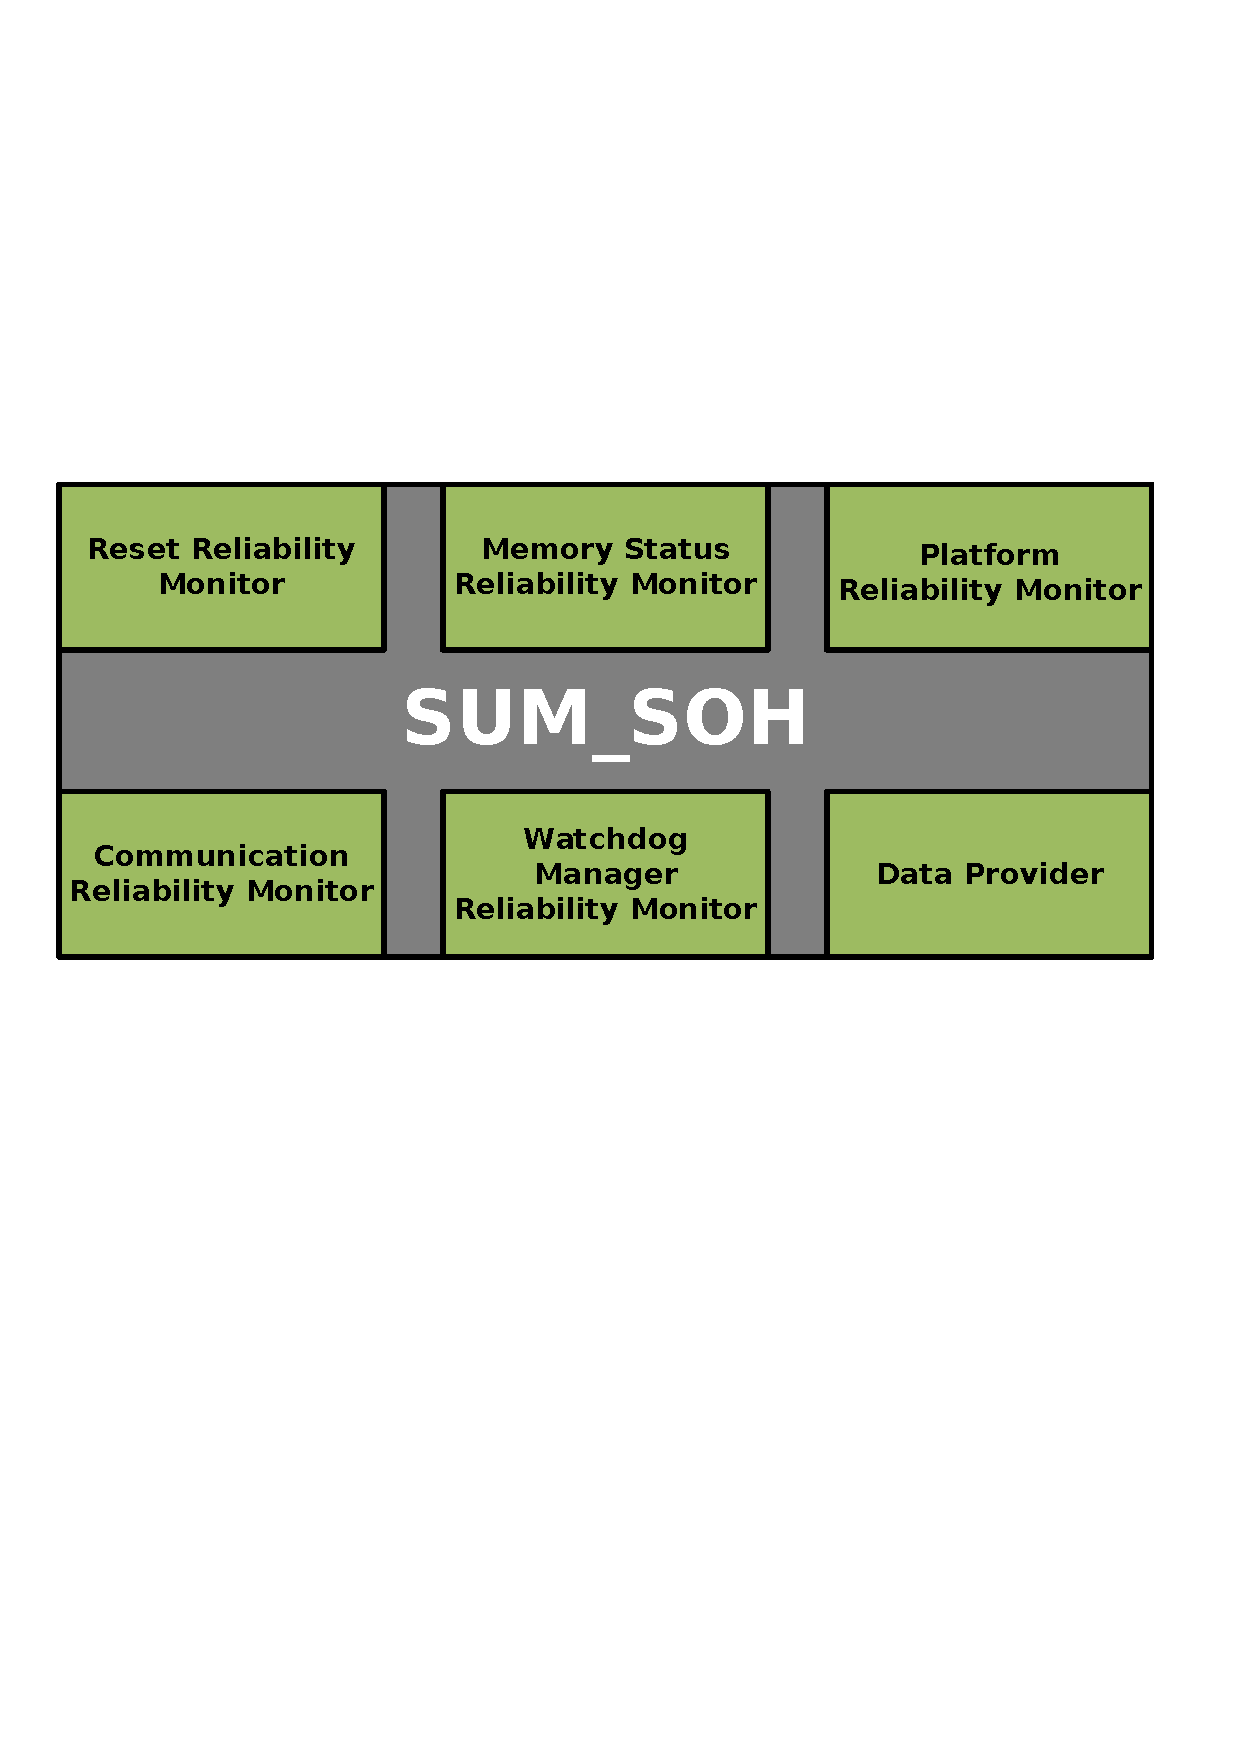
\includegraphics[scale=0.6]{images/Block_view}
	\caption{Inner structure of the system}
	\label{fig:Block_view}
\end{figure}

\section{Memory Types}
\label{subsection:Memory}

\Requirement{019}
{
To store the SUM\_SOH metrics four different types of memory are needed : 

\begin{itemize}
	\item RAM
	\item Non Cleared RAM
    \item Adaptable NVM
    \item Secure Cumulative NVM
\end{itemize}

Those types of memory shall be provided by the integrator. 
In partucular, for  Adaptable NVM and Secure Cumulative NVM the ECU should provide an NvM module that meets the GM definition for those two types.
Instead, for RAM and Non Cleared RAM types, the MemMap header file is generated using the MemMapGen generator present in RTA-CAR tool.
}
{
\Satisfies{SRS_SOH 013} \Satisfies{SRS_SOH 066} \Satisfies{SRS_SOH 067} \Satisfies{SRS_SOH 068}
}


\Requirement{058}
{
	For those counters not located in RAM, if their values changed and the battery voltage is in range, their values are saved in the NvM.
}
{
\Satisfies{SRS_SOH 027} \Satisfies{SRS_SOH 265}
}

\RequirementTag{SDD_SOH}{057}
\\
The memory type where the SUM_SOH detection counters are located shall be assigned as defined in the following table \ref{fig:memorytypes}.

\begin{figure}[htp]
\centering
	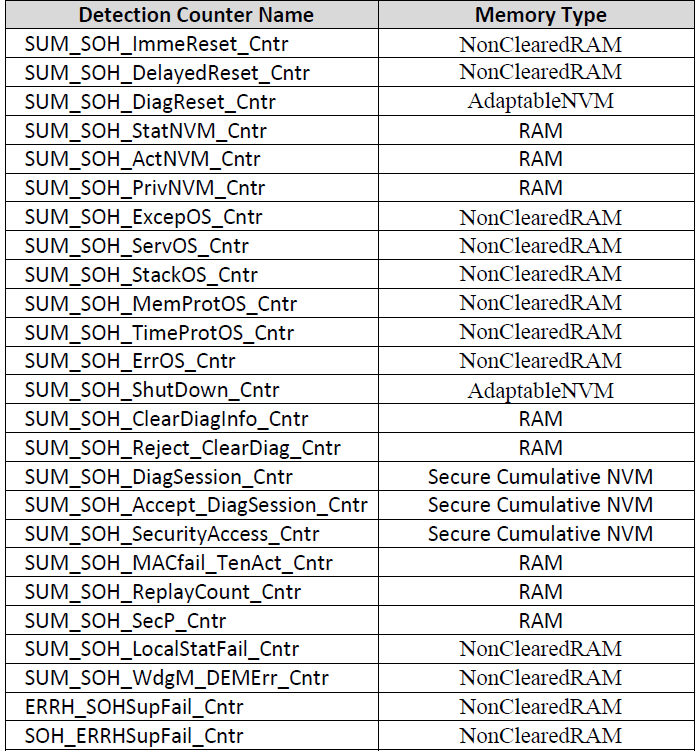
\includegraphics[scale=1]{images/memorytypes}
	\caption{Detector memory types}
	\label{fig:memorytypes}
\end{figure}
\Satisfies{SRS_SOH 029} \Satisfies{SRS_SOH 047} \Satisfies{SRS_SOH 066}



\clearpage 


\section{Filters}
\label{section:Filters}

There are two types of filter, the "Threshold" one checks if the number of events are above the threshold, the "Time window" insted checks if the number of events are above the threshold in a defined time span.

\UMLDiagram{generated/diagrams/filters}{SOH Filters}

\subsubsection{Threshold Filtering}

\Requirement{011}
{A 2-byte unsigned integer is used as detection counter to maintain a raw count of the detected events. Each detection counter shall reside in its respective memory and shall be initialized to a value of 0x0000 at ECU production.
 A 2-byte unsigned integer is used as DID counter to maintain a filtered count of the detected events. Each shall be stored in secure cumulative NVM. Each shall be initialized to a value of 0x0000 at ECU production. 
}
{
\Satisfies{SRS_SOH 028} \Satisfies{SRS_SOH 029} \Satisfies{SRS_SOH 030} \Satisfies{SRS_SOH 033} \Satisfies{SRS_SOH 041} \Satisfies{SRS_SOH 042}
}

\Requirement{014}
{Each detection counter will have a counter threshold calibration value associated with it}
{
\Satisfies{SRS_SOH 032}
}

\Requirement{015}
{Each detection counter and DID counter shall be cleared to a value of 0x0000 during execution of RID 0x02C0 Clear_SUM_SOH_logs.}
{
\Satisfies{SRS_SOH 031}
\Satisfies{SRS_SOH 043}
}

\Requirement{020}
{
In the case where the detection counter reaches its threshold count calibration, the following steps SUM\_SOH:
\begin{itemize}
	\item Increments the DID counter by one.
	\item Resets the detection counter to 0x0000 and starts a new detection cycle
\end{itemize}

Also, if the DID counter reaches its maximum value of 0xFFFE before read time, that value is retained until the next execution of RID 0x02C0 Clear\_SUM\_SOH\_logs.
}
{
\Satisfies{SRS_SOH 044} \Satisfies{SRS_SOH 045} 
}


\subsubsection{Threshold during a time window filtering}
This feature is described in the Architecture Design document.


\section{Reliability monitors}
\subsection{Reset Reliability monitor}

\Requirement{025}
{
The scope of this monitor is to track the occurrences of three types of reset : Immediate, Delayed and Diagnostic resets.
}
{
\Satisfies{SRS_SOH 071} \Satisfies{SRS_SOH 072} \Satisfies{SRS_SOH 079} \Satisfies{SRS_SOH 086} \Satisfies{SRS_SOH 022} 
}

\Requirement{026}
{
    \textbf{Immediate Reset Detector}
    
    
    To handle the Immediate reset a Time Window filter is used  with the following variables :
    
    \begin{itemize}
        \item Counter               : SUM_SOH_ImmeReset_Cntr
        \item Counter Threshold     : SUM_SOH_ImmeReset_Thresh
        \item Time Window           : SUM_SOH_ImmeReset_TW
        \item Time Window Threshold : SUM_SOH_ImmeReset_TW_Thresh
        \item DID                   : SUM_SOH_DID_ImmeReset_Cntr
    \end{itemize}
    
}
{
\Satisfies{SRS_SOH 073} \Satisfies{SRS_SOH 074} \Satisfies{SRS_SOH 075} \Satisfies{SRS_SOH 076} \Satisfies{SRS_SOH 077} \Satisfies{SRS_SOH 078} \Satisfies{SRS_SOH 226} \Satisfies{SRS_SOH 227}
}

\Requirement{027}
{
    \textbf{Delayed Reset Detector}
    
    
    To handle the Delayed reset a Time Window filter is used  with the following variables :
    
    
    \begin{itemize}
        \item Counter               : SUM_SOH_DelayedReset_Cntr
        \item Counter Threshold     : SUM_SOH_DelayedReset_Thresh
        \item Time Window           : SUM_SOH_DelayedReset_TW
        \item Time Window Threshold : SUM_SOH_DelayedReset_TW_Thresh
        \item DID                   : SUM_SOH_DID_DelayedReset_Cntr
    \end{itemize}
    
}
{
\Satisfies{SRS_SOH 080} \Satisfies{SRS_SOH 081} \Satisfies{SRS_SOH 082} \Satisfies{SRS_SOH 083}  \Satisfies{SRS_SOH 084} \Satisfies{SRS_SOH 085} \Satisfies{SRS_SOH 226} \Satisfies{SRS_SOH 227}
}

\Requirement{028}
{
    \textbf{Diagnostic Reset Detector}
    
    
    To handle the Diagnostic reset a Threshold filter is used  with the following variables :
    
    \begin{itemize}
        \item Counter               : SUM_SOH_DiagReset_Cntr
        \item Counter Threshold     : SUM_SOH_DiagReset_Thresh
        \item DID                   : SUM_SOH_DID_DiagReset_Cntr
    \end{itemize}
    
}
{
\Satisfies{SRS_SOH 087} \Satisfies{SRS_SOH 088}  \Satisfies{SRS_SOH 089} \Satisfies{SRS_SOH 090} \Satisfies{SRS_SOH 226} \Satisfies{SRS_SOH 227}
}

\Requirement{029}
{
The events about \textbf{Immediate} and \textbf{Delayed resets} are provided by SUM\_SUSD. \newline\newline
The \textbf{\code{Runnable_SOHResetReliabilityMonitor_ImmeDelayedReset}} handles the type of reset through the interface \code{SUSD_SOH_ResetOccured} and increments  of one unit the counter
\code{SSUM_SOH_ImmeReset_Cntr} or  \code{SSUM_SOH_DelayedReset_Cntr} based on the read value.\newline\newline
It calls the \code{SOH_Filter} on the activeted detector and if the DID has changed and if the battery voltage is in range, the DID is saved in the NvM.

}
{
\Satisfies{SRS_SOH 020} \Satisfies{SRS_SOH 235}
} 

\Requirement{030}
{
The events about \textbf{Diagnostic reset} are provided by SUM\_DIAG.\newline\newline 
The \textbf{\code{Runnable_SOHResetReliabilityMonitor_DiagReset}} handles them through the interface \code{DIAG_ECUResetRequest} and increments  of one unit the counter
\code{SUM_SOH_DiagReset_Cntr}.\newline\newline
It calls the \code{SOH_Filter} on the activeted detector and if the DID or the Counter have changed and if the battery voltage is in range, the DID and the Counter are saved in the NvM.

}
{
\Satisfies{SRS_SOH 029} \Satisfies{SRS_SOH 047} \Satisfies{SRS_SOH 027} \Satisfies{SRS_SOH 265} \Satisfies{SRS_SOH 086} \Satisfies{SRS_SOH 246}
}

\newpage

\subsection{Memory Status Reliability Monitor}
\Requirement{044}
{
The scope of this monitor is to track the occurrences of two types of faults : NvM and OS faults.
}
{
\Satisfies{SRS_SOH 091}
}

\RequirementTag{SDD_SOH}{045}
\newline

    \subsubsection{NVM Errors Detector}
    
    
    To handle the NVM faults, three different detectors based on a Time Window filter are used  with the following variables :\newline\newline
    
    \textbf{Status Failure/Integrity}
    \begin{itemize}
        \item Counter               : SUM_SOH_StatNVM_Cntr
        \item Counter Threshold     : SUM_SOH_StatNVM_Thresh
        \item Time Window           : SUM_SOH_StatNVM_TW
        \item Time Window Threshold : SUM_SOH_StatNVM_TW_Thresh
        \item DID                   : SUM_SOH_DID_StatNVM_Cntr
    \end{itemize}
    
    
    \textbf{Action Failure}
    \begin{itemize}
        \item Counter               : SUM_SOH_ActNVM_Cntr
        \item Counter Threshold     : SUM_SOH_ActNVM_Thresh
        \item Time Window           : SUM_SOH_ActNVM_TW
        \item Time Window Threshold : SUM_SOH_ActNVM_TW_Thresh
        \item DID                   : SUM_SOH_DID_ActNVM_Cntr
    \end{itemize}
    
    \textbf{Privilege}
    \begin{itemize}
        \item Counter               : SUM_SOH_PrivNVM_Cntr
        \item Counter Threshold     : SUM_SOH_PrivNVM_Thresh
        \item Time Window           : SUM_SOH_PrivNVM_TW
        \item Time Window Threshold : SUM_SOH_PrivNVM_TW_Thresh
        \item DID                   : SUM_SOH_DID_PrivNVM_Cntr
    \end{itemize}
    

{\Satisfies{SRS_SOH 091}\Satisfies{SRS_SOH 092}\Satisfies{SRS_SOH 093}\Satisfies{SRS_SOH 094}}
{\Satisfies{SRS_SOH 096}\Satisfies{SRS_SOH 097}\Satisfies{SRS_SOH 098}\Satisfies{SRS_SOH 099}}
{\Satisfies{SRS_SOH 100}\Satisfies{SRS_SOH 101}\Satisfies{SRS_SOH 102}\Satisfies{SRS_SOH 226} \Satisfies{SRS_SOH 227}}


\Requirement{046}
{
The failure events  are provided by SUM\_ERRH. \newline\newline
The \textbf{\code{Runnable_SOH_ERRH_BswEvent}} handles the faults through the interface \code{ERRH_E_BswEvent} and, based on the read value, increments  of one unit the related counter.
 
 
It calls the \code{SOH_Filter} on the activeted detector and if the DID has changed and if the battery voltage is in range, the DID is saved in the NvM.\newline\newline


The mapping between NVM Errors and detectors is the following :\newline

\begin{center}\begin{tabular}{|l|c|}
\hline
\textbf{Fault}                & \textbf{Detector}               \\ \hline
NVM\_E\_HARDWARE              &  Status Failure/Integrity       \\ \hline
NVM\_E\_QUEUE\_OVERFLOW     &  Status Failure/Integrity       \\ \hline
NVM\_E\_INTEGRITY\_FAILED           &  Status Failure/Integrity       \\ \hline
NVM\_E\_REQ\_FAILED       &  Action Failure                 \\ \hline
NVM\_E\_WRONG\_BLOCK\_ID      &  Action Failure                 \\ \hline
NVM\_E\_VERIFY\_FAILED        &  Action Failure                 \\ \hline
NVM\_E\_LOSS\_OF\_REDUNDANCY   &  Action Failure                 \\ \hline
NVM\_E\_WRITE\_PROTECTED      &  Privilege                      \\ \hline
\hline
\end{tabular}\end{center}

}
{
\Satisfies{SRS_SOH 095}  
} 

\Requirement{047}
{
SUM\_SOH allows to enable/disable each type of the failure events (and the relative detector) through the following configuration parameters: \newline


\begin{center}\begin{tabular}{|l|c|}
\hline
\textbf{Calibration Parameter}     & \textbf{Detector}               \\ \hline
SOH\_StatNvM\_SupportEnabled       &  Status Failure/Integrity       \\ \hline
SOH\_ActNvM\_SupportEnabled        &  Action Failure                 \\ \hline
SOH\_PrivNvM\_SupportEnabled       &  Privilege                      \\ \hline
\hline
\end{tabular}\end{center}


If the detector is disabled, the relative detection counter and DID counters of the corresponding class are permanently set to the reserved value 0xFFFF.

}
{
\Satisfies{SRS_SOH 103}  
} 
\subsubsection{OS Errors Detector}
\RequirementTag{SDD_SOH}{069}
\\
\\
The SUM\_SOH shall monitor the frequency of OS related errors and use the threshold during a time window filtering method to
check for these occurrences. The SUM\_SOH shall also implement a unique DID counter associated with each detection OS fault class

\vspace*{0.2in}

\textbf{Hardware Protection}
\begin{itemize}
    \item Counter               : SUM_SOH_ExcepOS_Cntr
    \item Counter Threshold     : SUM_SOH_ExcepOS_Thresh
    \item Time Window           : SUM_SOH_ExcepOS_TW 
    \item Time Window Threshold : SUM_SOH_ExcepOS_TW_Thresh 
    \item DID                   : SUM_SOH_DID_ExcepOS_Cntr
\end{itemize}

\textbf{Service Protection and Trusted Function}
\begin{itemize}
    \item Counter               : SUM_SOH_ServOS_Cntr
    \item Counter Threshold     : SUM_SOH_ServOS_Thresh
    \item Time Window           : SUM_SOH_ServOS_TW 
    \item Time Window Threshold : SUM_SOH_ServOS_TW_Thresh 
    \item DID                   : SUM_SOH_DID_ServOS_Cntr
\end{itemize}

\textbf{Stack Fault}
\begin{itemize}
    \item Counter               : SUM_SOH_StackOS_Cntr
    \item Counter Threshold     : SUM_SOH_StackOS_Thresh
    \item Time Window           : SUM_SOH_StackOS_TW 
    \item Time Window Threshold : SUM_SOH_StackOS_TW_Thresh 
    \item DID                   : SUM_SOH_DID_StackOS_Cntr
\end{itemize}

\textbf{Memory Protection}
\begin{itemize}
    \item Counter               : SUM_SOH_MemProtOS_Cntr
    \item Counter Threshold     : SUM_SOH_MemProtOS_Thresh
    \item Time Window           : SUM_SOH_MemProtOS_TW 
    \item Time Window Threshold : SUM_SOH_MemProtOS_TW_Thresh 
    \item DID                   : SUM_SOH_DID_MemProtOS_Cntr
\end{itemize}

\textbf{Time Protection}
\begin{itemize}
    \item Counter               : SUM_SOH_TimeProtOS_Cntr
    \item Counter Threshold     : SUM_SOH_TimeProtOS_Thresh
    \item Time Window           : SUM_SOH_TimeProtOS_TW 
    \item Time Window Threshold : SUM_SOH_TimeProtOS_TW_Thresh 
    \item DID                   : SUM_SOH_DID_TimeProtOS_Cntr
\end{itemize}

\textbf{Other OS Errors}
\begin{itemize}
    \item Counter               : SUM_SOH_ErrOS_Cntr
    \item Counter Threshold     : SUM_SOH_ErrOS_Thresh
    \item Time Window           : SUM_SOH_ErrOS_TW 
    \item Time Window Threshold : SUM_SOH_ErrOS_TW_Thresh 
    \item DID                   : SUM_SOH_DID_ErrOS_Cntr
\end{itemize}
\vspace*{0.2in}
\Satisfies{SRS_SOH 104} \Satisfies{SRS_SOH 105} \Satisfies{SRS_SOH 106} \Satisfies{SRS_SOH 108} \\
\Satisfies{SRS_SOH 109} \Satisfies{SRS_SOH 110} \Satisfies{SRS_SOH 111} \Satisfies{SRS_SOH 112} \\
\Satisfies{SRS_SOH 226} \Satisfies{SRS_SOH 227}

\Requirement{073}{
	Callback called by the OS in its ProtectionHook and ErrorHook
	to identify the OS Error type and update the proper event detector (counter + filter).
}{
	\Satisfies{SRS_SOH 114} \Satisfies{SRS_SOH 115}
}

\Requirement{067}
{
    The OS Errors shall be provided by ErrorHook and ProtectionHook Callbacks that are called in turn  by OS when one of its API fails.\newline

    The \textbf{\code{SOH_OS_Protection_ErrorHook_Callback}} is called by ErrorHook and ProtectionHook to report OS Error type to SUM\_SOH.\newline

    The mapping between OS Errors and detectors is the following :\newline

    \begin{center}\begin{tabular}{|l|c|}
    \hline
    \textbf{Fault}                & \textbf{Detector}               \\ \hline
    E_OS_PROTECTION_EXCEPTION   &  Hardware Protection       \\ \hline
    E_OS_SERVICEID     &  Service Protection / Trusted Function       \\ \hline
    E_OS_ILLEGAL_ADDRESS     &  Service Protection / Trusted Function       \\ \hline
    E_OS_MISSINGEND     &  Service Protection / Trusted Function       \\ \hline
    E_OS_DISABLEDINT     &  Service Protection / Trusted Function       \\ \hline
    E_OS_STACKFAULT           &  Stack Fault       \\ \hline
    E_OS_PROTECTION_MEMORY       &  Memory Protection                 \\ \hline
    E_OS_PROTECTION_TIME      &  Time Protection                 \\ \hline
    E_OS_PROTECTION_ARRIVAL        &  Time Protection                 \\ \hline
    E_OS_PROTECTION_LOCKED        &  Time Protection                 \\ \hline
    Others                     &  Other OS Errors                 \\ \hline
    \hline
    \end{tabular}\end{center}  
}
{
    \Satisfies{SRS_SOH 107} \Satisfies{SRS_SOH 113} \Satisfies{SRS_SOH 114}
}

\Requirement{068}
{
SUM\_SOH allows to enable/disable each type of the OS failure (and the relative detector) through the following configuration parameters: \newline


\begin{center}\begin{tabular}{|l|c|}
\hline
\textbf{Calibration Parameter}   & \textbf{Detector}            \\ \hline
SOH_ExcepOS_SupportEnabled       &  Hardware Protection    \\ \hline
SOH_ServOS_SupportEnabled        &  Service Protection / Trusted Function              \\ \hline
SOH_StackOS_SupportEnabled       &  Stack Fault                   \\ \hline
SOH_MemProtOS_SupportEnabled     &  Memory Protection              \\ \hline
SOH_TimeProtOS_SupportEnabled    &  Time Protection               \\ \hline
SOH_ErrOS_SupportEnabled         &  Other OS Errors                \\ \hline 
\hline
\end{tabular}\end{center}


If the detector is disabled, the relative detection counter and DID counters of the corresponding class are permanently set to the reserved value 0xFFFF.
}
{
    \Satisfies{SRS_SOH 115}
}


\subsection{Communication Reliability Monitor}
\label{subsection:CommunicationReliabilityMonitor}

\Requirement{059}
{
	The scope of this monitor is to keep track of the following communication-related events:
	\begin{itemize}
		\item Clear Diagnostic Information Request
		\item Diagnostic Session Control Request
		\item SecurityAccess (Service 0x27) Failures
		\item MAC Failures
		\item SecP Errors.
	\end{itemize}
}
{
\Satisfies{SRS_SOH 133}
}

\subsubsection{Clear Diagnostic Information Request}
\Requirement{060}
{
    \textbf{\textit{Clear Diagnostic Information Accepted Request} Detector}\\
    To handle the \textit{Clear Diagnostic Information Accepted Request} a Threshold filter is used  with the following variables:
    \begin{itemize}
        \item Counter               : SUM_SOH_ClearDiagInfo_Cntr
        \item Counter Threshold     : SUM_SOH_ClearDiagInfo_Thresh
        \item DID                   : SUM_SOH_DID_ClearDiagInfo_Cntr
    \end{itemize}
}
{
\Satisfies{SRS_SOH 134} \Satisfies{SRS_SOH 136} \Satisfies{SRS_SOH 137} \Satisfies{SRS_SOH 138} \Satisfies{SRS_SOH 139} \Satisfies{SRS_SOH 226} \Satisfies{SRS_SOH 227}
}

\Requirement{061}
{
    \textbf{\textit{Clear Diagnostic Information Rejected Request} Detector}\\
    To handle the \textit{Clear Diagnostic Information Rejected Request} a Threshold filter is used  with the following variables:
    \begin{itemize}
        \item Counter               : SUM_SOH_Reject_ClearDiag_Cntr
        \item Counter Threshold     : SUM_SOH_Reject_ClearDiag_Thresh
        \item DID                   : SUM_SOH_DID_Reject_ClearDiag_Cntr
    \end{itemize}
}
{
\Satisfies{SRS_SOH 140} \Satisfies{SRS_SOH 142} \Satisfies{SRS_SOH 143} \Satisfies{SRS_SOH 144} \Satisfies{SRS_SOH 145} \Satisfies{SRS_SOH 226} \Satisfies{SRS_SOH 227}
}

\Requirement{062}
{
	Both Clear Diagnostic Information Request events are provided by SUM_SSFM.

	The SSFM writes in SSFM_ClearDiagReq to notify the SOH about a Clear Diagnostic Information Request and triggers \code{Runnable_SOH_CommunicationReliabilityMonitor_ClearDiag()}.\\
	The ERRH can write the following values:
	\begin{itemize}
		\item 0x00		:	Default
		\item 0x01		:	Clear Diagnostic Request Approved, the SOH increases by one SUM_SOH_ClearDiagInfo_Cntr and calls \code{SOH_Filter()} for the \textit{Clear Diagnostic Information Accepted Request} Detector
		\item 0x02		:	Clear Diagnostic Request Rejected, the SOH increases by one SUM_SOH_Reject_ClearDiag_Cntr and calls \code{SOH_Filter()} for the \textit{Clear Diagnostic Information Rejected Request} Detector
		\item 0x03-0x0F	:	Invalid.
	\end{itemize}
}
{
\Satisfies{SRS_SOH 135} \Satisfies{SRS_SOH 141}  \Satisfies{SRS_SOH 239}
}


\subsubsection{Diagnostic Session Control Request}
\Requirement{063}
{
    \textbf{\textit{Diagnostic Session Control Request} Detector}\\
    To handle the \textit{Diagnostic Session Control Request} a Threshold filter is used  with the following variables:
    \begin{itemize}
        \item Counter               : SUM_SOH_DiagSession_Cntr
        \item Counter Threshold     : SUM_SOH_DiagSession_Thresh
        \item DID                   : SUM_SOH_DID_DiagSession_Cntr
    \end{itemize}
}
{
\Satisfies{SRS_SOH 146} \Satisfies{SRS_SOH 147} \Satisfies{SRS_SOH 148} \Satisfies{SRS_SOH 149} \Satisfies{SRS_SOH 150} \Satisfies{SRS_SOH 226} \Satisfies{SRS_SOH 227} \Satisfies{SRS_SOH 247}
}

The DIAG writes in DIAG_SOH_DiagSessionRequest to notify the SOH about a Diagnostic Session Request (service 0x10 subfunction 0x02) and triggers \code{Runnable_SOH_CommunicationReliabilityMonitor_DiagSession()}.\\
The DIAG can write the following values:
\begin{itemize}
	\item FALSE		:	No Diagnostic Session Request (initial value)
	\item TRUE		:	Diagnostic Session Requested, the SOH increases by one SUM_SOH_DiagSession_Cntr and calls \code{SOH_Filter()} for the \textit{Diagnostic Session Control Request} Detector.
\end{itemize}

\Requirement{064}
{
    \textbf{\textit{Accepted Diagnostic Session Control Request} Detector}\\
    To handle the \textit{Accepted Diagnostic Session Control Request} a Threshold filter is used  with the following variables:
    \begin{itemize}
        \item Counter               : SUM_SOH_Accept_DiagSession_Cntr
        \item Counter Threshold     : SUM_SOH_Accept_DiagSession_Thresh
        \item DID                   : SUM_SOH_DID_Accept_DiagSession_Cntr
    \end{itemize}
}
{
\Satisfies{SRS_SOH 151} \Satisfies{SRS_SOH 152} \Satisfies{SRS_SOH 153} \Satisfies{SRS_SOH 154} \Satisfies{SRS_SOH 155} \Satisfies{SRS_SOH 226} \Satisfies{SRS_SOH 227}
}

The Accept Diagnostic Session Control Request event is provided by BswM.

The BswM writes in the mode port DiagnosticReprogrammingRequest to notify the SOH about an Accepted Diagnostic Session Request and triggers \code{Runnable_SOH_CommunicationReliabilityMonitor_AcceptDiagSession()}.\\
The BswM can write the following modes:
\begin{itemize}
	\item 0x00		:	SUM_REPREQ_ACTIVE, the SOH increases by one SUM_SOH_Accept_DiagSession_Cntr and calls \code{SOH_Filter()} for the \textit{Accepted Diagnostic Session Control Request} Detector
	\item 0x01		:	SUM_REPREQ_INACTIVE (initial value).
\end{itemize}


\subsubsection{SecurityAccess (Service 0x27) Failures}
\Requirement{065}
{
    \textbf{\textit{SecurityAccess (Service 0x27) Failures} Detector}\\
    To handle the \textit{SecurityAccess (Service 0x27) Failures} a Threshold filter is used  with the following variables:
    \begin{itemize}
        \item Counter               : SUM_SOH_SecurityAccess_Cntr
        \item Counter Threshold     : SUM_SOH_SecurityAccess_Thresh
        \item DID                   : SUM_SOH_DID_SecurityAccess_Cntr
    \end{itemize}
}
{
\Satisfies{SRS_SOH 156} \Satisfies{SRS_SOH 157} \Satisfies{SRS_SOH 158} \Satisfies{SRS_SOH 159} \Satisfies{SRS_SOH 160} \Satisfies{SRS_SOH 226} \Satisfies{SRS_SOH 227} \Satisfies{SRS_SOH 245}
}

The SecurityAccess (Service 0x27) Failures events are provided by SSC.

The SSC writes in SSC_SOH_SecurityAccessError to notify the SOH about a SecurityAccess CompareKey (servcie 0x27) Failure and triggers \code{Runnable_SOH_CommunicationReliabilityMonitor_SecurityAccess()}.\\
The SSC can write the following values:
\begin{itemize}
	\item FALSE		:	No SecurityAccess failures (initial value)
	\item TRUE		:	A SecurityAccess failure, the SOH increases by one SUM_SOH_SecurityAccess_Cntr and calls \code{SOH_Filter()} for the \textit{SecurityAccess (Service 0x27) Failures} Detector.
\end{itemize}


\subsubsection{MAC Failures}
\Requirement{066}
{
    \textbf{\textit{MAC Failures Types 1 and 2} Detector}\\
    To handle the \textit{MAC Failures Types 1 and 2} a Time Window filter is used  with the following variables:
    \begin{itemize}
        \item Counter               : SUM_SOH_MACfail_TenAct_Cntr
        \item Counter Threshold     : SUM_SOH_MACfail_TenAct_Thresh
        \item Time Window           : SUM_SOH_MACfail_TenAct_TW
        \item Time Window Threshold : SUM_SOH_MACfail_TenAct_TW_Thresh
        \item DID                   : SUM_SOH_DID_MACfail_TenAct_Cntr
    \end{itemize}
}
{
\Satisfies{SRS_SOH 166} \Satisfies{SRS_SOH 167} \Satisfies{SRS_SOH 168} \Satisfies{SRS_SOH 169} \Satisfies{SRS_SOH 170} \Satisfies{SRS_SOH 171} \Satisfies{SRS_SOH 172} \Satisfies{SRS_SOH 226} \Satisfies{SRS_SOH 227}
}

\Requirement{070}
{
    \textbf{\textit{MAC Failures Type 3} Detector}\\
    To handle the \textit{MAC Failures Type 3} a Time Window filter is used  with the following variables:
    \begin{itemize}
        \item Counter               : SUM_SOH_ReplayCount_Cntr
        \item Counter Threshold     : SUM_SOH_ReplayCount_Thresh
        \item Time Window           : SUM_SOH_ReplayCount_TW
        \item Time Window Threshold : SUM_SOH_ReplayCount_TW_Thresh
        \item DID                   : SUM_SOH_DID_ReplayCount_Cntr
    \end{itemize}
}
{
\Satisfies{SRS_SOH 173} \Satisfies{SRS_SOH 174} \Satisfies{SRS_SOH 175} \Satisfies{SRS_SOH 176} \Satisfies{SRS_SOH 177} \Satisfies{SRS_SOH 178} \Satisfies{SRS_SOH 179} \Satisfies{SRS_SOH 226} \Satisfies{SRS_SOH 227}
}


\Requirement{071}
{
	Respect to the SOH initialization, \textit{MAC Failures Type 3} logs are delayed a number of seconds defined in the 1-byte calibration value SUM_SOH_ReplayCount_Start_Thresh.\\
	This is a startup delay that allows the MAC counters to establish an initial synchronization before the detectors start counting errors.\\
	Until the delay does not expire, the value of the boolean flag SUM_SOH_ReplayCount_Start_Status is FALSE.\\
	\code{Runnable_SOH_CommunicationReliabilityMonitor_MacFailType3Delay()} runs periodically to check the elapsing time and - if the delay expired - flags SUM_SOH_ReplayCount_Start_Status to TRUE.
	
}
{
\Satisfies{SRS_SOH 180} \Satisfies{SRS_SOH 181} \Satisfies{SRS_SOH 182}
}


\Requirement{072}
{
	The three types of MAC Failures events are provided by SSC.

	The SSC writes in SSC_E_SecureMessageMonitoringEvents to notify the SOH about a MAC Failure not related to SecP failures and triggers \code{Runnable_SOH_CommunicationReliabilityMonitor_MacFailType123()}.\\
	The SSC can write the following values:
	\begin{itemize}
		\item 0x00		:	SSC_ERR_NO_Event (initial value)
		\item 0x01		:	SSC_ERR_MAC_Active, if the MACVerify failure event occurs when using the Active Counter while the tentative Counter state was invalid upon receipt of an authenticated message. In this case, SUM_SOH  increases by one SUM_SOH_MACfail_TenAct_Cntr and calls \code{SOH_Filter()} for the \textit{MAC Failures Types 1 and 2} Detector
		\item 0x02		:	SSC_ERR_Tentative_Active, if the MACVerify failure event occurs while using the Active Counter after failed MAC verification using the Tentative Counter. In this case, SUM_SOH increases by one SUM_SOH_MACfail_TenAct_Cntr and calls \code{SOH_Filter()} for the \textit{MAC Failures Types 1 and 2} Detector
		\item 0x03		:	SSC_ERR_Low_Tentative, if the 64-bit counter received in a Counter Sync Message is not accepted by the receiver due to its value being less than or equal to the Active Counter. In this case, if SUM_SOH_ReplayCount_Start_Status is TRUE, SUM_SOH increases by one SUM_SOH_ReplayCount_Cntr and calls \code{SOH_Filter()} for the \textit{MAC Failures Type 3} Detector.
	\end{itemize}
}
{
\Satisfies{SRS_SOH 161} \Satisfies{SRS_SOH 162} \Satisfies{SRS_SOH 163} \Satisfies{SRS_SOH 164} \Satisfies{SRS_SOH 165} \Satisfies{SRS_SOH 182} \Satisfies{SRS_SOH 244}
}


\subsubsection{SecP Errors}
\Requirement{052}
{
    \textbf{\textit{SecP Errors} Detector}\\
    To handle the \textit{SecP Errors} a Time Window filter is used  with the following variables:
    \begin{itemize}
        \item Counter               : SUM_SOH_SecP_Cntr
        \item Counter Threshold     : SUM_SOH_SecP_Thresh
        \item Time Window           : SUM_SOH_SecP_TW
        \item Time Window Threshold : SUM_SOH_SecP_TW_Thresh
        \item DID                   : SUM_SOH_DID_SecP_Cntr
    \end{itemize}
}
{
\Satisfies{SRS_SOH 183} \Satisfies{SRS_SOH 184} \Satisfies{SRS_SOH 186} \Satisfies{SRS_SOH 187} \Satisfies{SRS_SOH 188} \Satisfies{SRS_SOH 189} \Satisfies{SRS_SOH 190} \Satisfies{SRS_SOH 226} \Satisfies{SRS_SOH 227}
}

\Requirement{054}
{
The SOH component includes the RPort RP\_ErrorStatus for receiving the HSM error notification from BswM. This Mode User Port refers to the Mode Declaration Group SECP\_Error\_Status and SOH reports the HSM error codes using the following mapping with SECP\_Error\_Status modes:
%Table
\begin{longtable}{|l|l|l|}
\hline
\begin{minipage}{0.38\linewidth}\raggedright\vspace{.75ex}\textbf{HSM Error Code}\vspace{.75ex}\end{minipage} & \begin{minipage}{0.15\linewidth}\raggedright\vspace{.75ex}\textbf{Enumeration}\vspace{.75ex}\end{minipage} & \begin{minipage}{0.38\linewidth}\raggedright\vspace{.75ex}\textbf{Mode Declaration}\vspace{.75ex}\end{minipage}\\
\hline\hline
\endfirsthead
\hline
\begin{minipage}{0.38\linewidth}\raggedright\vspace{.75ex}\textbf{HSM Error Code}\vspace{.75ex}\end{minipage} & \begin{minipage}{0.15\linewidth}\raggedright\vspace{.75ex}\textbf{Enumeration}\vspace{.75ex}\end{minipage} & \begin{minipage}{0.38\linewidth}\raggedright\vspace{.75ex}\textbf{Mode Declaration}\vspace{.75ex}\end{minipage}\\
\hline\hline
\endhead
\hline
\endfoot
\hline
\endlastfoot
\begin{minipage}{0.38\linewidth}\raggedright\vspace{.75ex}ERC\_BUSY\vspace{.75ex}\end{minipage} & \begin{minipage}{0.15\linewidth}\raggedright\vspace{.75ex}0x02\vspace{.75ex}\end{minipage} & \begin{minipage}{0.38\linewidth}\raggedright\vspace{.75ex}SUM\_ERC\_BUSY\vspace{.75ex}\end{minipage}\\\hline
\begin{minipage}{0.38\linewidth}\raggedright\vspace{.75ex}ERC\_GENERAL\_FAILURE\vspace{.75ex}\end{minipage} & \begin{minipage}{0.15\linewidth}\raggedright\vspace{.75ex}0xFF\vspace{.75ex}\end{minipage} & \begin{minipage}{0.38\linewidth}\raggedright\vspace{.75ex}SUM\_ERC\_GENERAL\_FAILURE\vspace{.75ex}\end{minipage}\\\hline
\begin{minipage}{0.38\linewidth}\raggedright\vspace{.75ex}ERC\_KEY\_EMPTY\vspace{.75ex}\end{minipage} & \begin{minipage}{0.15\linewidth}\raggedright\vspace{.75ex}0x12\vspace{.75ex}\end{minipage} & \begin{minipage}{0.38\linewidth}\raggedright\vspace{.75ex}SUM\_ERC\_KEY\_EMPTY\vspace{.75ex}\end{minipage}\\\hline
\begin{minipage}{0.38\linewidth}\raggedright\vspace{.75ex}ERC\_KEY\_INVALID\vspace{.75ex}\end{minipage} & \begin{minipage}{0.15\linewidth}\raggedright\vspace{.75ex}0x11\vspace{.75ex}\end{minipage} & \begin{minipage}{0.38\linewidth}\raggedright\vspace{.75ex}SUM\_ERC\_KEY\_INVALID\vspace{.75ex}\end{minipage}\\\hline
\begin{minipage}{0.38\linewidth}\raggedright\vspace{.75ex}ERC\_KEY\_NOT\_AVAILABLE\vspace{.75ex}\end{minipage} & \begin{minipage}{0.15\linewidth}\raggedright\vspace{.75ex}0x10\vspace{.75ex}\end{minipage} & \begin{minipage}{0.38\linewidth}\raggedright\vspace{.75ex}SUM\_ERC\_KEY\_NOT\_AVAILABLE\vspace{.75ex}\end{minipage}\\\hline
\begin{minipage}{0.38\linewidth}\raggedright\vspace{.75ex}ERC\_KEY\_UPDATE\_ERROR\vspace{.75ex}\end{minipage} & \begin{minipage}{0.15\linewidth}\raggedright\vspace{.75ex}0x31\vspace{.75ex}\end{minipage} & \begin{minipage}{0.38\linewidth}\raggedright\vspace{.75ex}SUM\_ERC\_KEY\_UPDATE\_ERROR\vspace{.75ex}\end{minipage}\\\hline
\begin{minipage}{0.38\linewidth}\raggedright\vspace{.75ex}ERC\_KEY\_WRITE\_PROTECTED\vspace{.75ex}\end{minipage} & \begin{minipage}{0.15\linewidth}\raggedright\vspace{.75ex}0x30\vspace{.75ex}\end{minipage} & \begin{minipage}{0.38\linewidth}\raggedright\vspace{.75ex}SUM\_ERC\_KEY\_WRITE\_PROTECTED\vspace{.75ex}\end{minipage}\\\hline
\begin{minipage}{0.38\linewidth}\raggedright\vspace{.75ex}ERC\_MEMORY\_FAILURE\vspace{.75ex}\end{minipage} & \begin{minipage}{0.15\linewidth}\raggedright\vspace{.75ex}0x50\vspace{.75ex}\end{minipage} & \begin{minipage}{0.38\linewidth}\raggedright\vspace{.75ex}SUM\_ERC\_MEMORY\_FAILURE\vspace{.75ex}\end{minipage}\\\hline
\begin{minipage}{0.38\linewidth}\raggedright\vspace{.75ex}ERC\_NO\_DEBUGGING\vspace{.75ex}\end{minipage} & \begin{minipage}{0.15\linewidth}\raggedright\vspace{.75ex}0x60\vspace{.75ex}\end{minipage} & \begin{minipage}{0.38\linewidth}\raggedright\vspace{.75ex}SUM\_ERC\_NO\_DEBUGGING\vspace{.75ex}\end{minipage}\\\hline
\begin{minipage}{0.38\linewidth}\raggedright\vspace{.75ex}ERC\_NO\_ERROR\vspace{.75ex}\end{minipage} & \begin{minipage}{0.15\linewidth}\raggedright\vspace{.75ex}0x00\vspace{.75ex}\end{minipage} & \begin{minipage}{0.38\linewidth}\raggedright\vspace{.75ex}SUM\_ERC\_NO\_ERROR\vspace{.75ex}\end{minipage}\\\hline
\begin{minipage}{0.38\linewidth}\raggedright\vspace{.75ex}ERC\_NO\_SECURE\_BOOT\vspace{.75ex}\end{minipage} & \begin{minipage}{0.15\linewidth}\raggedright\vspace{.75ex}0x20\vspace{.75ex}\end{minipage} & \begin{minipage}{0.38\linewidth}\raggedright\vspace{.75ex}SUM\_ERC\_NO\_SECURE\_BOOT\vspace{.75ex}\end{minipage}\\\hline
\begin{minipage}{0.38\linewidth}\raggedright\vspace{.75ex}ERC\_SEQUENCE\_ERROR\vspace{.75ex}\end{minipage} & \begin{minipage}{0.15\linewidth}\raggedright\vspace{.75ex}0x01\vspace{.75ex}\end{minipage} & \begin{minipage}{0.38\linewidth}\raggedright\vspace{.75ex}SUM\_ERC\_SEQUENCE\_ERROR\vspace{.75ex}\end{minipage}\\\hline
\begin{minipage}{0.38\linewidth}\raggedright\vspace{.75ex}ERC\_RNG\_SEED\vspace{.75ex}\end{minipage} & \begin{minipage}{0.15\linewidth}\raggedright\vspace{.75ex}0x40\vspace{.75ex}\end{minipage} & \begin{minipage}{0.38\linewidth}\raggedright\vspace{.75ex}SUM\_ERC\_RNG\_SEED\vspace{.75ex}\end{minipage}\\\hline
\end{longtable}

For the correct error code reporting SOH assumes that BswM configuration includes the definition of:

\begin{itemize}
	\item a Mode Switch Port to be connected to RP\_ErrorStatus;
	\item a Mode Request Port to receive mode change requests from Cry module;
	\item a Rule for each mode change notification to SOH. 	
\end{itemize}

For all the values different than 0x00, the SOH increases by one SUM_SOH_SecP_Cntr and calls \code{SOH_Filter()} for the \textit{SecP Errors} Detector.
}
{
\Satisfies{SRS_SOH 185} \Satisfies{SRS_SOH 251}
}


\subsection{Watchdog Manager Reliability Monitor}
\label{subsec:wdgmreliabilitymonitor}

\Requirement{094}
{
The scope of this monitor is to track the occurrences of: Failed Local Supervisions of Supervised Entities (except ERRH and SOH), WDGM\_E\_SUPERVISION or WDGM\_E\_SET\_MODE errors, and SUM\_ERRH Failed Local Supervisions.
}
{
\Satisfies{SRS_SOH 191} \Satisfies{SRS_SOH 192} \Satisfies{SRS_SOH 193} \Satisfies{SRS_SOH 200} \Satisfies{SRS_SOH 216}
}

\Requirement{095}
{
    \textbf{Local Supervision Failures Detector}
    
    
    To handle the Failed Local Supervision, a Time Window filter is used  with the following variables :
    
    \begin{itemize}
        \item Counter               : SUM_SOH_LocalStatFail_Cntr
        \item Counter Threshold     : SUM_SOH_LocalStatFail_Thresh
        \item Time Window           : SUM_SOH_LocalStatFail_TW
        \item Time Window Threshold : SUM_SOH_LocalStatFail_TW_Thresh
        \item DID                   : SUM_SOH_DID_LocalStatFail_Cntr
    \end{itemize}
    
}
{
\Satisfies{SRS_SOH 194} \Satisfies{SRS_SOH 195} \Satisfies{SRS_SOH 196} \Satisfies{SRS_SOH 197} \Satisfies{SRS_SOH 198} \Satisfies{SRS_SOH 199} \Satisfies{SRS_SOH 226} \Satisfies{SRS_SOH 227}
}

\Requirement{098}
{
The WdgM provides the events of Failed Local Supervisions of Supervised Entities through the corresponding WdgM\_LocalMode interface.
In particular, for each Supervised Entity, the WdgM generates a port whose interface is WdgM\_LocalMode.\newline
For each supervised entity (except ERRH and SOH), there exists a \textbf{\code{Runnable_WdgMReliabilityMonitor_FailedLocalSupervision_\<Supervised\_Entity\_name\>}} which is invoked when one of the following three events occurs:
\begin{enumerate}
\item The local supervision status (read at the corresponding SOH\_WdgM\_IndividualMode port) of the supervised entity transitions from SUPERVISION\_OK (0) to SUPERVISION\_FAILED (1).
\item The local supervision status (read at the corresponding SOH\_WdgM\_IndividualMode port) of the supervised entity transitions from SUPERVISION\_OK (0) to SUPERVISION\_EXPIRED (2).
\item The local supervision status (read at the corresponding SOH\_WdgM\_IndividualMode port) of the supervised entity transitions from SUPERVISION\_FAILED (1) to SUPERVISION\_EXPIRED (2).
\end{enumerate}

These runnables increment the counter \code{SUM\_SOH\_LocalStatFail\_Cntr} that they share. They also call the \code{SOH_Filter} and if the \code{SUM_SOH_DID_LocalStatFail_Cntr} is changed and the battery voltage is in range, the \code{SUM_SOH_DID_LocalStatFail_Cntr} is saved into the NvM.

The SOH guarantees a synchronized access to \code{SUM\_SOH\_LocalStatFail\_Cntr} and the other shared variables (that the runnables access in the \code{SOH_Filter} function)  by defining proper \code{EXCLUSIVE-AREAS}.
}
{
\Satisfies{SRS_SOH 027} \Satisfies{SRS_SOH 265} \Satisfies{SRS_SOH 029} \Satisfies{SRS_SOH 038} \Satisfies{SRS_SOH 047} \Satisfies{SRS_SOH 192} \Satisfies{SRS_SOH 193} \Satisfies{SRS_SOH 194} \Satisfies{SRS_SOH 249} \Satisfies{SRS_SOH 250}
}

\Requirement{096}
{
    \textbf{WdgM DEM Supervision Errors Detector}
    
    
    To handle the WDGM\_E\_SUPERVISION and WDGM\_E\_SET\_MODE errors, a Time Window filter is used  with the following variables :
    
    
    \begin{itemize}
        \item Counter               : SUM_SOH_WdgM_DEMErr_Cntr
        \item Counter Threshold     : SUM_SOH_WdgM_DEMErr_Thresh
        \item Time Window           : SUM_SOH_WdgM_DEMErr_TW
        \item Time Window Threshold : SUM_SOH_WdgM_DEMErr_TW_Thresh
        \item DID                   : SUM_SOH_DID_WdgM_DEMErr_Cntr
    \end{itemize}
    
}
{
\Satisfies{SRS_SOH 200} \Satisfies{SRS_SOH 201} \Satisfies{SRS_SOH 202} \Satisfies{SRS_SOH 203} \Satisfies{SRS_SOH 204} \Satisfies{SRS_SOH 205} \Satisfies{SRS_SOH 226} \Satisfies{SRS_SOH 227}
}

\Requirement{099}
{
The events  of WDGM\_E\_SUPERVISION and WDGM\_E\_SET\_MODE are provided by the ERRH. \newline
The \textbf{\code{Runnable_SOH_ERRH_BswEvent}} is invoked when the value at the ERRH\_E\_BswEvent interface changes. 

If one of the following events occurs:

\begin{itemize}
\item WDGM\_E\_SUPERVISION
\item WDGM\_E\_SET\_MODE
\end{itemize}


the runnable increments the \code{SUM_SOH_WdgM_DEMErr_Cntr}. It also calls the \code{SOH_Filter} and if the \code{SUM_SOH_DID_WdgM_DEMErr_Cntr} is changed and the battery voltage is in range, the \code{SUM_SOH_DID_WdgM_DEMErr_Cntr} is saved into the NvM.
}
{
\Satisfies{SRS_SOH 027} \Satisfies{SRS_SOH 265} \Satisfies{SRS_SOH 029} \Satisfies{SRS_SOH 038} \Satisfies{SRS_SOH 047} \Satisfies{SRS_SOH 200} \Satisfies{SRS_SOH 228} \Satisfies{SRS_SOH 229} \Satisfies{SRS_SOH 238}
}

\Requirement{097}
{
    \textbf{SUM_ERRH Local Supervision Detector}
    
    
    To handle the SUM\_ERRH local supervision failures a Time Window filter is used  with the following variables :
    
    
    \begin{itemize}
        \item Counter               : SOH_ERRHSupFail_Cntr
        \item Counter Threshold     : SOH_ERRHSupFail_Thresh
        \item Time Window           : SOH_ERRHSupFail_TW
        \item Time Window Threshold : SOH_ERRHSupFail_TW_Thresh
        \item DID                   : SUM_SOH_DID_ERRHSupFail_Cntr
    \end{itemize}
    
}
{
\Satisfies{SRS_SOH 218} \Satisfies{SRS_SOH 219} \Satisfies{SRS_SOH 220} \Satisfies{SRS_SOH 221} \Satisfies{SRS_SOH 222} \Satisfies{SRS_SOH 223} \Satisfies{SRS_SOH 226} \Satisfies{SRS_SOH 227}
}

\Requirement{100}
{
The WdgM provides the events of Failed Local Supervisions of the ERRH through the corresponding WdgM\_LocalMode interface.
The \textbf{\code{Runnable_SOH_WdgMReliabilityMonitor_ERRHFailedLocalSupervision}} is is invoked when one of the following three events occurs:
\begin{enumerate}
\item The local supervision status (read at the SOH\_WdgM\_IndividualMode\_Errh interface) of the ERRH transitions from SUPERVISION\_OK (0) to SUPERVISION\_FAILED (1).
\item The local supervision status (read at the SOH\_WdgM\_IndividualMode\_Errh interface) of the ERRH transitions from SUPERVISION\_OK (0) to SUPERVISION\_EXPIRED (2).
\item The local supervision status (read at the SOH\_WdgM\_IndividualMode\_Errh interface) of the ERRH transitions from SUPERVISION\_FAILED (1) to SUPERVISION\_EXPIRED (2).
\end{enumerate}

This runnable increments the \code{SOH_ERRHSupFail_Cntr} and calls the \code{SOH_Filter}. If the \code{SUM_SOH_DID_ERRHSupFail_Cntr} is changed and the battery voltage is in range, the \code{SUM_SOH_DID_ERRHSupFail_Cntr} is saved into the NvM.
The \code{ERRH_Local_Supervision_Status} field of the DID 0xF093, will be instead updated directly in the DID function which, when called, reads the ERRH Local Supervision Status.
}
{
\Satisfies{SRS_SOH 027} \Satisfies{SRS_SOH 265} \Satisfies{SRS_SOH 029}  \Satisfies{SRS_SOH 038} \Satisfies{SRS_SOH 047} \Satisfies{SRS_SOH 217} \Satisfies{SRS_SOH 218} \Satisfies{SRS_SOH 224} \Satisfies{SRS_SOH 225} \Satisfies{SRS_SOH 249}
}  

\Requirement{101}
{
    \textbf{SUM\_SOH Local Supervision Detector}
    
     SUM\_ERRH implements this detector. However, to guarantee its proper behaviour the SUM\_SOH executes the logic needed to update the corresponding WdgM\_LocalSupervision port interface.
    
}
{
\Satisfies{SRS_SOH 207}\Satisfies{SRS_SOH 262}
}

\subsection{Platform Reliability Monitor}
\label{subsection:PlatformReliabilityMonitor}
This feature is described in the Architecture Design document.

\subsection{Data Provider}
SUM\_SOH  provides data regarding monitored events via DIDs allocated for the SUM\_SOH and SUM\_ERRH.


\section{RID 0x02C0 Clear SOH Logs}

\Requirement{038}
{
Through the UDS Routine 0x02C0 (Clear SUM\_SOH Logs) the tester can clear detectors, timers, DIDs and counters for all the SOH monitors. 
This routine implements only the SubFunction 0x1 (Start Routine) with 2 unsigned bytes as Option Record.

The accepted values for the Option Record are :
\begin{itemize}
\item 0xF08F : clear DID F08F metrics
\item 0xF090 : clear DID F090 metrics
\item 0xF091 : clear DID F091 metrics
\item 0xF092 : clear DID F092 metrics
\item 0xF093 : clear DID F093 metrics
\item 0xF094 : asks the ERRH to clear DID F094 metrics
\item 0xFFFF : clear all metrics
\end{itemize}

This RID must be created by the user in the DCM module so that after BSW generation the interface \textbf{RoutineServices\_Clear\_SUM\_SOH\_logs} is available.
}
{
\Satisfies{SRS_SOH 040} \Satisfies{SRS_SOH 069} \Satisfies{SRS_SOH 266}
}



\Requirement{039}
{
SUM\_SOH implements the \textbf{Runnable\_SOH\_RIDClearLogs} that is the Server part of the interface \textit{RoutineServices\_Clear\_SUM\_SOH\_logs}. It's called through
an Operation Invoked Event when the \textit{Start Routine} for the Routine 0x02C0 (Clear SUM\_SOH Logs) is invoked through the UDS protocol.
It clears the needed metrics based on the Option Record received value. 

The runnable behaviour is described in the diagram \ref{diagram:generated/diagrams/rid} .

}
{
\Satisfies{SRS_SOH 031} \Satisfies{SRS_SOH 043} \Satisfies{SRS_SOH 044} \Satisfies{SRS_SOH 056} \Satisfies{SRS_SOH 060} \Satisfies{SRS_SOH 061} \Satisfies{SRS_SOH 069} \Satisfies{SRS_SOH 266}
}

\Requirement{102} 
{ 
When the DCM calls the RID with Option Record values 0xF094 or 0xFFFF, the SUM\_SOH invokes a client operation service in the SUM\_ERRH (Acting as a server) to clean all the metrics related to SUM\_SOH Local Supervision Detector implemented at the ERRH side. To complete the RID 0x02C0 routine the SUM\_SOH shall interact with the SUM\_ERRH through the Client-Server interface SOH\_ERRH\_RID\_Clear\_Logs where SUM\_ERRH acts as a Server. }
{
\Satisfies{SRS_SOH 260}
\Satisfies{SRS_SOH 261}
}

\UMLDiagram{generated/diagrams/rid}{Runnable\_SOH\_RIDClearLogs}

\section{DID Counters}
\subsection{DID 0xF08F: SUM_SOH Reset Reliability Monitor}

\Requirement{031}
{
It shall export the results of reset  monitoring events that occur in an ECU. 
They are the following 2-byte unsigned integer :

\begin{itemize}
\item	SUM\_SOH\_DID\_ImmeReset\_Cntr
\item	SUM\_SOH\_DID\_DelayedReset\_Cntr
\item	SUM\_SOH\_DID\_DiagReset\_Cntr
\end{itemize}

}
{
\Satisfies{SRS_SOH 034}
}



Through operation invoked events those values are passed to the DCM .Four Runnables are used :

\Requirement{040}
{
\textbf{\code{Runnable_SOH_DID_F08F_Data_ImmeReset_Cntr}} to pass  SUM\_SOH\_DID\_ImmeReset\_Cntr.
}
{
\Satisfies{SRS_SOH 034}
}

\Requirement{041}
{
\textbf{\code{Runnable_SOH_DID_F08F_Data_DiagReset_Cntr}} to pass SUM\_SOH\_DID\_DiagReset\_Cntr.
}
{
\Satisfies{SRS_SOH 034}
}

\Requirement{042}
{
\textbf{\code{Runnable_SOH_DID_F08F_Data_DelayedReset_Cntr}} to pass SUM\_SOH\_DID\_DelayedReset\_Cntr.
} 
{
\Satisfies{SRS_SOH 034}
}

\Requirement{043}
{
\textbf{\code{Runnable_SOH_DID_F08F_CheckRead}} to allow the read.
}
{
\Satisfies{SRS_SOH 034}
}
 

\subsection{DID 0xF090: SUM_SOH Memory Status Reliability Monitor}

\Requirement{032}
{
It shall maintain the results of monitoring NVM production errors and OS errors that occur in an ECU.

\begin{itemize}
\item	SUM\_SOH\_DID\_StatNVM\_Cntr
\item	SUM\_SOH\_DID\_ActNVM\_Cntr
\item	SUM\_SOH\_DID\_PrivNVM\_Cntr
\item	SUM\_SOH\_DID\_ExcepOS\_Cntr
\item	SUM\_SOH\_DID\_ServOS\_Cntr
\item	SUM\_SOH\_DID\_StackOS\_Cntr
\item	SUM\_SOH\_DID\_MemProtOS\_Cntr
\item	SUM\_SOH\_DID\_TimeProtOS\_Cntr
\item	SUM\_SOH\_DID\_ErrOS\_Cntr
\end{itemize}
}
{
\Satisfies{SRS_SOH 035} \Satisfies{SRS_SOH 112} \Satisfies{SRS_SOH 113} \Satisfies{SRS_SOH 114}
}

Through operation invoked events those values are passed to the DCM .Ten Runnables are used :
\Requirement{048}
{
\textbf{\code{Runnable_SOH_DID_F090_Data_StatNVM_Cntr}} to pass  SUM\_SOH\_DID\_StatNVM\_Cntr.
}
{
\Satisfies{SRS_SOH 035}
}

\Requirement{049}
{
\textbf{\code{Runnable_SOH_DID_F090_Data_ActNVM_Cntr}} to pass  SUM\_SOH\_DID\_ActNVM\_Cntr.
}
{
\Satisfies{SRS_SOH 035}
}

\Requirement{050}
{
\textbf{\code{Runnable_SOH_DID_F090_Data_PrivNVM_Cntr}} to pass  SUM\_SOH\_DID\_PrivNVM\_Cntr.
}
{
\Satisfies{SRS_SOH 035}
}

\Requirement{051}
{
\textbf{\code{Runnable_SOH_DID_F090_Data_ExcepOS_Cntr}} to pass  SUM\_SOH\_DID\_ExcepOS\_Cntr.
}
{
\Satisfies{SRS_SOH 035}
}

\Requirement{083}
{
\textbf{\code{Runnable_SOH_DID_F090_Data_ServOS_Cntr}} to pass  SUM\_SOH\_DID\_ServOS\_Cntr.
}
{
\Satisfies{SRS_SOH 035}
}

\Requirement{053}
{
\textbf{\code{Runnable_SOH_DID_F090_Data_StackOS_Cntr}} to pass  SUM\_SOH\_DID\_StackOS\_Cntr.
}
{
\Satisfies{SRS_SOH 035}
}

\Requirement{085}
{
\textbf{\code{Runnable_SOH_DID_F090_Data_MemProtOS_Cntr}} to pass  SUM\_SOH\_DID\_MemProtOS\_Cntr.
}
{
\Satisfies{SRS_SOH 035}
}

\Requirement{055}
{
\textbf{\code{Runnable_SOH_DID_F090_Data_TimeProtOS_Cntr}} to pass  SUM\_SOH\_DID\_TimeProtOS\_Cntr.
}
{
\Satisfies{SRS_SOH 035}
}

\Requirement{056}
{
\textbf{\code{Runnable_SOH_DID_F090_Data_ErrOS_Cntr}} to pass  SUM\_SOH\_DID\_ErrOS\_Cntr.
}
{
\Satisfies{SRS_SOH 035}
}

\Requirement{084}
{
\textbf{\code{Runnable_SOH_DID_F090_CheckRead}} to allow the read.
}
{
\Satisfies{SRS_SOH 035}
}



\subsection{DID 0xF091: SUM_SOH Platform Reliability Monitor}
This feature is described in the Architecture Design document.

\subsection{DID 0xF092: SUM_SOH Communication Reliability Monitor}

\Requirement{034}
{
It shall maintain the results of monitoring communication related events.

\begin{itemize}
\item	SUM\_SOH\_DID\_ClearDiagInfo\_Cntr
\item	SUM\_SOH\_DID\_Reject_ClearDiag\_Cntr
\item	SUM\_SOH\_DID\_DiagSession\_Cntr
\item	SUM\_SOH\_DID\_Accept_DiagSession\_Cntr
\item	SUM\_SOH\_DID\_SecurityAccess\_Cntr
\item	SUM\_SOH\_DID\_MACfail_TenAct\_Cntr
\item	SUM\_SOH\_DID\_ReplayCount\_Cntr
\item	SUM\_SOH\_DID\_SecP\_Cntr
\end{itemize}
Each one of them is a 2-byte unsigned integer.

They are used to update  the DCM DID 0xF092 by Runnable\_SOH\_DID\_F092 through an operation invoked event. 
}
{
\Satisfies{SRS_SOH 037}
}

Through operation invoked events those values are passed to the DCM .Four Runnables are used :

\Requirement{074}
{
\textbf{\code{Runnable_SOH_DID_F092_Data_ClearDiagInfo_Cntr}} to pass  SUM\_SOH\_DID\_ClearDiagInfo\_Cntr.
}
{
\Satisfies{SRS_SOH 037}
}

\Requirement{075}
{
\textbf{\code{Runnable_SOH_DID_F092_Data_Reject_ClearDiag_Cntr}} to pass  SUM\_SOH\_DID\_Reject\_ClearDiag\_Cntr.
}
{
\Satisfies{SRS_SOH 037}
}

\Requirement{076}
{
\textbf{\code{Runnable_SOH_DID_F092_Data_DiagSession_Cntr}} to pass  SUM\_SOH\_DID\_DiagSession\_Cntr.
}
{
\Satisfies{SRS_SOH 037}
}

\Requirement{077}
{
\textbf{\code{Runnable_SOH_DID_F092_Data_Accept_DiagSession_Cntr}} to pass  SUM\_SOH\_DID\_Accept\_DiagSession\_Cntr.
}
{
\Satisfies{SRS_SOH 037}
}

\Requirement{078}
{
\textbf{\code{Runnable_SOH_DID_F092_Data_SecurityAccess_Cntr}} to pass  SUM\_SOH\_DID\_SecurityAccess\_Cntr.
}
{
\Satisfies{SRS_SOH 037}
}

\Requirement{079}
{
\textbf{\code{Runnable_SOH_DID_F092_Data_MACfail_TenAct_Cntr}} to pass  SUM\_SOH\_DID\_MACfail\_TenAct\_Cntr.
}
{
\Satisfies{SRS_SOH 037}
}

\Requirement{080}
{
\textbf{\code{Runnable_SOH_DID_F092_Data_ReplayCount_Cntr}} to pass  SUM\_SOH\_DID\_ReplayCount\_Cntr.
}
{
\Satisfies{SRS_SOH 037}
}

\Requirement{081}
{
\textbf{\code{Runnable_SOH_DID_F092_Data_SecP_Cntr}} to pass  SUM\_SOH\_DID\_SecP\_Cntr.
}
{
\Satisfies{SRS_SOH 037}
}

\Requirement{082}
{
\textbf{\code{Runnable_SOH_DID_F092_CheckRead}} to allow the read.
}
{
\Satisfies{SRS_SOH 034}
}

\subsection{DID 0xF093: SUM_SOH Watchdog Manager Reliability Monitor}

\Requirement{035}
{
It shall maintain the results of monitoring communication related events.

\begin{itemize}
\item	SUM\_SOH\_DID\_LocalStatFail\_Cntr
\item	SUM\_SOH\_DID\_WdgM_DEMErr\_Cntr
\item	SUM\_SOH\_DID\_ERRHSupFail\_Cntr
\item	ERRH\_Local\_Supervision\_Status
\end{itemize}
Each one of them is a 2-byte unsigned integer except ERRH\_Local\_Supervision\_Status is 1-byte unsigned integer.\newline

}
{
\Satisfies{SRS_SOH 038}
}

Through operation invoked events those values are passed to the DCM .Five Runnables are used :

\Requirement{104}
{
\textbf{\code{Runnable_SOH_DID_F093_Data_LocalStatFail_Cntr}} to pass  SUM\_SOH\_DID\_LocalStatFail\_Cntr
}
{
\Satisfies{SRS_SOH 038}
}

\Requirement{105}
{
\textbf{\code{Runnable_SOH_DID_F093_Data_Data_WdgM_DEMErr_Cntr}} to pass  SUM\_SOH\_DID\_WdgM_DEMErr\_Cntr
}
{
\Satisfies{SRS_SOH 038}
}

\Requirement{106}
{
\textbf{\code{Runnable_SOH_DID_F093_Data_ERRHSupFail_Cntr}} to pass  SUM\_SOH\_DID\_ERRHSupFail\_Cntr
}
{
\Satisfies{SRS_SOH 038}
}

\Requirement{107}
{
\textbf{\code{Runnable_SOH_DID_F093_Data_ERRH_Local_Supervision_Status}} to pass  ERRH\_Local\_Supervision\_Status
}
{
\Satisfies{SRS_SOH 038}
}

\Requirement{108}
{
\textbf{\code{Runnable_SOH_DID_F093_CheckRead}} to allow the read.
}
{
\Satisfies{SRS_SOH 038}
}

\section{Configuration}
\label{sec:Configuration}

\Requirement{112}
{
SUM\_SOH is a SWC within the context of AUTOSAR.
It consists of static files and generated files.
SUM\_SOH configuration is done the same way as for standard BSW modules.
A parameter definition file is included with the module which allows users to configure the available parameters.
The generated files change based on the configuration.


For default values of calibration thresholds SOH is referring to the SDV-8002.
Configuration parameters shall be pre-compile, in other words the ECU behavior modification requires
a reflash of the complete application software.
}
{\Satisfies{SRS_SOH 070} \Satisfies{SRS_SOH 254} \Satisfies{SRS_SOH 255} \Satisfies{SRS_SOH 256}}

\subsection{Included Containers}
\begin{longtable}{|l|l|l|}
\hline
\begin{minipage}{0.25\linewidth}\raggedright\vspace{.75ex}\textbf{Name}\vspace{.75ex}\end{minipage} & \begin{minipage}{0.17\linewidth}\raggedright\vspace{.75ex}\textbf{Multiplicity}\vspace{.75ex}\end{minipage} & \begin{minipage}{0.50\linewidth}\raggedright\vspace{.75ex}\textbf{Scope / Dependency}\vspace{.75ex}\end{minipage}\\
\hline\hline
\endfirsthead
\hline
\begin{minipage}{0.25\linewidth}\raggedright\vspace{.75ex}\textbf{Name}\vspace{.75ex}\end{minipage} & \begin{minipage}{0.17\linewidth}\raggedright\vspace{.75ex}\textbf{Multiplicity}\vspace{.75ex}\end{minipage} & \begin{minipage}{0.50\linewidth}\raggedright\vspace{.75ex}\textbf{Scope / Dependency}\vspace{.75ex}\end{minipage}\\
\hline\hline
\endhead
\hline
\endfoot
\hline
\endlastfoot
\begin{minipage}{0.25\linewidth}\raggedright\vspace{.75ex}SOHGeneral\vspace{.75ex}\end{minipage} & \begin{minipage}{0.17\linewidth}\raggedright\vspace{.75ex}1..1\vspace{.75ex}\end{minipage} & \begin{minipage}{0.50\linewidth}\raggedright\vspace{.75ex}General configuration parameters of the SOH\vspace{.75ex}\end{minipage}\\\hline
\begin{minipage}{0.25\linewidth}\raggedright\vspace{.75ex}SUSDConfigSet\vspace{.75ex}\end{minipage} & \begin{minipage}{0.17\linewidth}\raggedright\vspace{.75ex}1..1\vspace{.75ex}\end{minipage} & \begin{minipage}{0.50\linewidth}\raggedright\vspace{.75ex}This container contains the configuration parameters and sub containers of the SOH module supporting multiple SWC configuration sets\vspace{.75ex}\end{minipage}\\\hline
\end{longtable}

\subsection{SOHGeneral}
\label{subsection:SOHGen}

{   \ConfigurationParameter{SOH_PermitExecution_Mask}
    {Mask that can be OR'd with the value supplied by PermitExecution to set any "don't care" bits to '1'.}
    {1..1}
    {ECUC-INTEGER-PARAM-DEF}
    {0..255}
    {190}
}

{
    \ConfigurationParameter{SOH_RunnableSOHMainPeriod}
    {Time in sec, for the periodicity of the Runnable_SOH_Main.}
    {1..1}
    {ECUC-INTEGER-PARAM-DEF}
    {0.001..0.2}
    {0.1}
}

\Requirement{036}
{
    \ConfigurationParameter{SohGenerateInitRunnable}
    {This parameter, when configured to TRUE, generates a periodic Runnable Entity that is useful for calling the SOH_Init() function just once.}
    {1..1}
    {ECUC-BOOLEAN-PARAM-DEF}
    {NA}
    {0}
}


{
    \ConfigurationParameter{SohInitFuncPeriodicity}
    {This parameter is used to specify the time in ms for the periodicity of the runnable Runnable_SOH_Init.}
    {0..1}
    {ECUC-FLOAT-PARAM-DEF}
    {1.0...5000.0}
    {1000.0}
}

{
\Satisfies{SRS_SOH 259}
}


{\ConfigurationParameter{SOH\_StatNvM\_SupportEnabled}
{This parameter is used to enable the Nvm Status Failure/Integrity Error class and the relative detector.}
{1..1}
{ECUC-BOOLEAN-PARAM-DEF}
{NA}
{1}}

{\ConfigurationParameter{SOH\_ActNvM\_SupportEnabled}
{This parameter is used to enable the Nvm Action Failure Error class and the relative detector.}
{1..1}
{ECUC-BOOLEAN-PARAM-DEF}
{NA}
{1}}

{\ConfigurationParameter{SOH\_PrivNvM\_SupportEnabled}
{This parameter is used to enable the Nvm Privilege class and the relative detector.}
{1..1}
{ECUC-BOOLEAN-PARAM-DEF}
{NA}
{1}}

{
    \ConfigurationParameter{SOH_ExcepOS_SupportEnabled}
    {This parameter is used to enable the OS Hardware Protection Action Failure Error class and the relative detector.}
    {1..1}
    {ECUC-BOOLEAN-PARAM-DEF}
    {NA}
    {true}
}


{
    \ConfigurationParameter{SOH_ServOS_SupportEnabled}
    {This parameter is used to enable the OS Service Protection / Trusted Function Action Failure Error class and the relative detector.}
    {1..1}
    {ECUC-BOOLEAN-PARAM-DEF}
    {NA}
    {true}
}

{
    \ConfigurationParameter{SOH_StackOS_SupportEnabled}
    {This parameter is used to enable the OS Stack Fault class and the relative detector.}
    {1..1}
    {ECUC-BOOLEAN-PARAM-DEF}
    {NA}
    {true}
}

{
    \ConfigurationParameter{SOH_MemProtOS_SupportEnabled}
    {This parameter is used to enable the OS Memory Protection Failure Error class and the relative detector.}
    {1..1}
    {ECUC-BOOLEAN-PARAM-DEF}
    {NA}
    {true}
}


{
    \ConfigurationParameter{SOH_TimeProtOS_SupportEnabled}
    {This parameter is used to enable the OS Time Protection Action Failure Error class and the relative detector.}
    {1..1}
    {ECUC-BOOLEAN-PARAM-DEF}
    {NA}
    {true}
}


{
    \ConfigurationParameter{SOH_ErrOS_SupportEnabled}
    {This parameter is used to enable the OS Other OS Errors Action Failure Error class and the relative detector.}
    {1..1}
    {ECUC-BOOLEAN-PARAM-DEF}
    {NA}
    {true}
}



{\ConfigurationParameter{SOH\_RID\_02C0\_SOH\_Clear\_Log\_Reference}
{Reference to DCM RID 0x02C0 SOH Clear Logs}
{1..1}
{ECUC-REFERENCE-DEF}
{NA}
{-}
\label{sec:confparamautosar}

{\ConfigurationParameter{SOH\_ImmediateDelayed\_SupportEnabled}
{It allows to enable (disable) the Immediate Reset Detector and Delayed Reset Detector in Reset Reliability monitor.}
{1..1}
{ECUC-REFERENCE-DEF}
{NA}
{TRUE}

{\ConfigurationParameter{SOH\_DiagnosticReset\_SupportEnabled}
{It allows to enable (disable) the Diagnostic Reset Detector in Reset Reliability monitor.}
{1..1}
{ECUC-REFERENCE-DEF}
{NA}
{TRUE}

{\ConfigurationParameter{SOH\_ClearDiagnosticInformation\_SupportEnabled}
{It allows to enable (disable) the Clear Diagnostic Information Accepted Request Detector and Clear Diagnostic Information Rejected Request Detector in Communication Reliability Monitor.}
{1..1}
{ECUC-REFERENCE-DEF}
{NA}
{TRUE}

{\ConfigurationParameter{SOH\_DiagnosticSessionControl\_SupportEnabled}
{It allows to enable (disable) the Diagnostic Session Control Request Detector and Accepted Diagnostic Session Control Request Detector in Communication Reliability Monitor.}
{1..1}
{ECUC-REFERENCE-DEF}
{NA}
{TRUE}

{\ConfigurationParameter{SOH\_SecurityAccessFailures\_SupportEnabled}
{It allows to enable (disable) the SecurityAccess (Service 0x27) Failures Detector in Communication Reliability Monitor.}
{1..1}
{ECUC-REFERENCE-DEF}
{NA}
{TRUE}

{\ConfigurationParameter{SOH\_MACFailures\_SupportEnabled}
{It allows to enable (disable) the MAC Failures Types 1 and 2 Detector and MAC Failures Type 3 Detector in Communication Reliability Monitor.}
{1..1}
{ECUC-REFERENCE-DEF}
{NA}
{TRUE}

{\ConfigurationParameter{SOH\_SecPErrors\_SupportEnabled}
{It allows to enable (disable) the SecP Errors Detector in Communication Reliability Monitor.}
{1..1}
{ECUC-REFERENCE-DEF}
{NA}
{TRUE}

{\ConfigurationParameter{SOH\_LocalSupervisionFailures\_SupportEnabled}
{It allows to enable (disable) the Local Supervision Failures Detector in Watchdog Manager Reliability Monitor. }
{1..1}
{ECUC-REFERENCE-DEF}
{NA}
{TRUE}

{\ConfigurationParameter{SOH\_WdgMDEMSupervisionErrors\_SupportEnabled}
{It allows to enable (disable) the WdgM DEM Supervision Errors Detector in Watchdog Manager Reliability Monitor.}
{1..1}
{ECUC-REFERENCE-DEF}
{NA}
{TRUE}

{\ConfigurationParameter{SOH\_ERRHLocalSupervision\_SupportEnabled}
{It allows to enable (disable) the SUM_ERRH Local Supervision Detector in Watchdog Manager Reliability Monitor.}
{1..1}
{ECUC-REFERENCE-DEF}
{NA}
{TRUE}

{\ConfigurationParameter{ERRH\_SOHLocalSupervision\_SupportEnabled}
{It allows to enable (disable) the SUM_SOH Local Supervision Detector implemented by the ERRH.}
{1..1}
{ECUC-REFERENCE-DEF}
{NA}
{TRUE}

{\ConfigurationParameter{SOH\_ShutdownDelay\_SupportEnabled}
{It allows to enable (disable) the Shutdown Delay Detector in Platform Reliability Monitor.}
{1..1}
{ECUC-REFERENCE-DEF}
{NA}
{TRUE}



\subsection{SOHConfigSet}
\label{subsection:SOHConfigSet}

\subsubsection{SOH\_ResetReliabilityMonitor}
This container includes the configuration parameters needed for the Reset Reliability Monitor detectors.


\paragraph{SOH\_ImmediateReset}
{\ConfigurationParameter{SUM_SOH_ImmeReset_Thresh_Init}
{Initial value of SUM_SOH_ImmeReset_Thresh}
{1..1}
{-}
{-..-}
{1}}

{\ConfigurationParameter{SUM_SOH_ImmeReset_TW_Thresh_Init}
{Initial value of SUM_SOH_ImmeReset_TW_Thresh}
{1..1}
{-}
{-..-}
{3600}}

{\ConfigurationParameter{SOH\_NvMImmResetDID\_Reference}
{Reference to the NVM DID Block}
{1..1}
{ECUC-REFERENCE-DEF}
{NA}
{-}}

{\ConfigurationParameter{SOH\_DID\_F08F\_ImmResetData\_Reference}
{Reference to DCM ImmReset Data}
{1..1}
{ECUC-REFERENCE-DEF}
{NA}
{-}}

\paragraph{SOH\_DelayedReset}

{\ConfigurationParameter{SUM_SOH_DelayedReset_Thresh_Init}
{Initial value of SUM_SOH_DelayedReset_Thresh}
{1..1}
{-}
{-..-}
{1}}

{\ConfigurationParameter{SUM_SOH_DelayedReset_TW_Thresh_Init}
{Initial value of SUM_SOH_DelayedReset_TW_Thresh}
{1..1}
{-}
{-..-}
{3600}}

{\ConfigurationParameter{SOH\_NvMDelayedResetDID\_Reference}
{Reference to the NVM DID Block}
{1..1}
{ECUC-REFERENCE-DEF}
{NA}
{-}}

{\ConfigurationParameter{SOH\_DID\_F08F\_DelayedResetData\_Reference}
{Reference to DCM DelayedReset Data}
{1..1}
{ECUC-REFERENCE-DEF}
{NA}
{-}}


\paragraph{SOH\_DiagnosticReset}

{\ConfigurationParameter{SUM_SOH_DiagReset_Thresh_Init}
{Initial value SUM_SOH_DiagReset_Thresh}
{1..1}
{-}
{-..-}
{1}}

{\ConfigurationParameter{SOH\_NvMDiagResetCntr\_Reference}
{Reference to the NVM Counter Block}
{1..1}
{ECUC-REFERENCE-DEF}
{NA}
{-}}

{\ConfigurationParameter{SOH\_NvMDiagResetDID\_Reference}
{Reference to the NVM DID Block}
{1..1}
{ECUC-REFERENCE-DEF}
{NA}
{-}}

{\ConfigurationParameter{SOH\_DID\_F08F\_DiagResetData\_Reference}
{Reference to DCM DiagReset Data}
{1..1}
{ECUC-REFERENCE-DEF}
{NA}
{-}}

\subsubsection{SOH\_MemoryStatusReliabilityMonitor}
This container includes the configuration parameters needed for the Memory Status Monitor detectors.

\underline{SOH\_NVMErrorsDetector}\newline
This container includes the configuration containers needed for the NVM Error detectors.

\paragraph{SOH\_StatusNVM}

{\ConfigurationParameter{SUM_SOH_StatNVM_Thresh_Init}
{Initial value of SUM_SOH_StatNVM_Thresh}
{1..1}
{-}
{-..-}
{1}}

{\ConfigurationParameter{SUM_SOH_StatNVM_TW_Thresh_Init}
{Initial value of SUM_SOH_StatNVM_TW_Thresh}
{1..1}
{-}
{-..-}
{3600}}

{\ConfigurationParameter{SOH\_NvMStatNVMDID\_Reference}
{Reference to the NVM DID Block}
{1..1}
{ECUC-REFERENCE-DEF}
{NA}
{-}}

{\ConfigurationParameter{SOH\_DID\_F090\_StatusNVM\_Reference}
{Reference to DCM StatusNVM Data}
{1..1}
{ECUC-REFERENCE-DEF}
{NA}
{-}}

\paragraph{SOH\_ActNVM}
{\ConfigurationParameter{SUM_SOH_ActNVM_Thresh_Init}
{Initial value of SUM_SOH_ActNVM_Thresh}
{1..1}
{-}
{-..-}
{1}}

{\ConfigurationParameter{SUM_SOH_ActNVM_TW_Thresh_Init}
{Initial value of SUM_SOH_ActNVM_TW_Thresh}
{1..1}
{-}
{-..-}
{3600}}

{\ConfigurationParameter{SOH\_NvMActNVMDID\_Reference}
{Reference to the NVM DID Block}
{1..1}
{ECUC-REFERENCE-DEF}
{NA}
{-}}

{\ConfigurationParameter{SOH\_DID\_F090\_ActNVM\_Reference}
{Reference to DCM ActNVM Data}
{1..1}
{ECUC-REFERENCE-DEF}
{NA}
{-}}

\paragraph{SOH\_PrivNVM}
{\ConfigurationParameter{SUM_SOH_PrivNVM_Thresh_Init}
{Initial value of SUM_SOH_PrivNVM_Thresh}
{1..1}
{-}
{-..-}
{1}}

{\ConfigurationParameter{SUM_SOH_PrivNVM_TW_Thresh_Init}
{Initial value of SUM_SOH_PrivNVM_TW_Thresh}
{1..1}
{-}
{-..-}
{3600}}

{\ConfigurationParameter{SOH\_NvMPrivNVMDID\_Reference}
{Reference to the NVM DID Block}
{1..1}
{ECUC-REFERENCE-DEF}
{NA}
{-}}

{\ConfigurationParameter{SOH\_DID\_F090\_PrivNVM\_Reference}
{Reference to DCM PrivNVM Data}
{1..1}
{ECUC-REFERENCE-DEF}
{NA}
{-}}


\underline{SOH\_OSErrorsDetector}\newline
The following configuration parameters are used to set the initial threshold value for each OS error class detection counter and their related time windows.
\vspace*{0.1in}

\paragraph{SOH_ExcepOS}
{\ConfigurationParameter{SUM_SOH_ExcepOS_Thresh_Init}
{Initial value of SUM_SOH_ExcepOS_Thresh}
{1..1}
{-}
{-..-}
{1}}

{\ConfigurationParameter{SUM_SOH_ExcepOS_TW_Thresh_Init}
{Initial value of SUM_SOH_ExcepOS_TW_Thresh}
{1..1}
{-}
{-..-}
{3600}}

{\ConfigurationParameter{SOH\_NvMExcepOSDID\_Reference}
{Reference to the NVM DID Block}
{1..1}
{ECUC-REFERENCE-DEF}
{NA}
{-}}

{\ConfigurationParameter{SOH\_DID\_F090\_ExcepOS\_Reference}
{Reference to DCM ExcepOS Data}
{1..1}
{ECUC-REFERENCE-DEF}
{NA}
{-}}


\paragraph{SOH_ServOS}
{\ConfigurationParameter{SUM_SOH_ServOS_Thresh_Init}
{Initial value of SUM_SOH_ServOS_Thresh}
{1..1}
{-}
{-..-}
{1}}

{\ConfigurationParameter{SUM_SOH_ServOS_TW_Thresh_Init}
{Initial value of SUM_SOH_ServOS_TW_Thresh}
{1..1}
{-}
{-..-}
{3600}}

{\ConfigurationParameter{SOH\_NvMServOSDID\_Reference}
{Reference to the NVM DID Block}
{1..1}
{ECUC-REFERENCE-DEF}
{NA}
{-}}

{\ConfigurationParameter{SOH\_DID\_F090\_ServOS\_Reference}
{Reference to DCM ServOS Data}
{1..1}
{ECUC-REFERENCE-DEF}
{NA}
{-}}

\paragraph{SOH_StackOS}
{\ConfigurationParameter{SUM_SOH_StackOS_Thresh_Init}
{Initial value of SUM_SOH_StackOS_Thresh}
{1..1}
{-}
{-..-}
{1}}

{\ConfigurationParameter{SUM_SOH_StackOS_TW_Thresh_Init}
{Initial value of SUM_SOH_StackOS_TW_Thresh}
{1..1}
{-}
{-..-}
{3600}}

{\ConfigurationParameter{SOH\_NvMStackOSDID\_Reference}
{Reference to the NVM DID Block}
{1..1}
{ECUC-REFERENCE-DEF}
{NA}
{-}}

{\ConfigurationParameter{SOH\_DID\_F090\_StackOS\_Reference}
{Reference to DCM StackOS Data}
{1..1}
{ECUC-REFERENCE-DEF}
{NA}
{-}}

\paragraph{SOH_MemProtOS}
{\ConfigurationParameter{SUM_SOH_MemProtOS_Thresh_Init}
{Initial value of SUM_SOH_MemProtOS_Thresh}
{1..1}
{-}
{-..-}
{1}}

{\ConfigurationParameter{SUM_SOH_MemProtOS_TW_Thresh_Init}
{Initial value of SUM_SOH_MemProtOS_TW_Thresh}
{1..1}
{-}
{-..-}
{3600}}

{\ConfigurationParameter{SOH\_NvMMemProtOSDID\_Reference}
{Reference to the NVM DID Block}
{1..1}
{ECUC-REFERENCE-DEF}
{NA}
{-}}

{\ConfigurationParameter{SOH\_DID\_F090\_MemProtOS\_Reference}
{Reference to DCM MemProtOS Data}
{1..1}
{ECUC-REFERENCE-DEF}
{NA}
{-}}

\paragraph{SOH_TimeProtOS}
{\ConfigurationParameter{SUM_SOH_TimeProtOS_Thresh_Init}
{Initial value of SUM_SOH_TimeProtOS_Thresh}
{1..1}
{-}
{-..-}
{1}}

{\ConfigurationParameter{SUM_SOH_TimeProtOS_TW_Thresh_Init}
{Initial value of SUM_SOH_TimeProtOS_TW_Thresh}
{1..1}
{-}
{-..-}
{3600}}

{\ConfigurationParameter{SOH\_NvMTimeProtOSDID\_Reference}
{Reference to the NVM DID Block}
{1..1}
{ECUC-REFERENCE-DEF}
{NA}
{-}}

{\ConfigurationParameter{SOH\_DID\_F090\_TimeProtOS\_Reference}
{Reference to DCM TimeProtOS Data}
{1..1}
{ECUC-REFERENCE-DEF}
{NA}
{-}}

\paragraph{SOH_ErrOS}
{\ConfigurationParameter{SUM_SOH_ErrOS_Thresh_Init}
{Initial value of SUM_SOH_ErrOS_Thresh}
{1..1}
{-}
{-..-}
{1}}

{\ConfigurationParameter{SUM_SOH_ErrOS_TW_Thresh_Init}
{Initial value of SUM_SOH_ErrOS_TW_Thresh}
{1..1}
{-}
{-..-}
{3600}}

{\ConfigurationParameter{SOH\_NvMErrOSDID\_Reference}
{Reference to the NVM DID Block}
{1..1}
{ECUC-REFERENCE-DEF}
{NA}
{-}}

{\ConfigurationParameter{SOH\_DID\_F090\_ErrOS\_Reference}
{Reference to DCM ErrOS Data}
{1..1}
{ECUC-REFERENCE-DEF}
{NA}
{-}}

{\ConfigurationParameter{SUM_SOH_ShutDown_Thresh_Init}
{Initial value of SUM_SOH_ShutDown_Thresh}
{1..1}
{-}
{-..-}
{1}}

{\ConfigurationParameter{SUM_SOH_ShutDown_Timer_Thresh_Init}
{Initial value of SUM_SOH_ShutDown_Timer_Thresh}
{1..1}
{-}
{-..-}
{60}}


\subsubsection{SOH_CommunicationReliabilityMonitor}
This container includes the configuration parameters needed for the Communication Reliability Monitor detectors. Here organized by events.

\paragraph{SOH_ClearDiagInfo}

{\ConfigurationParameter{SUM_SOH_ClearDiagInfo_Thresh_Init}
{Initial value of SUM_SOH_ClearDiagInfo_Thresh}
{1..1}
{-}
{-..-}
{1}}

{\ConfigurationParameter{SOH\_NvMClearDiagInfoDID\_Reference}
{Reference to the NVM DID Block}
{1..1}
{ECUC-REFERENCE-DEF}
{NA}
{-}}

{\ConfigurationParameter{SOH\_DID\_F092\_ClearDiagInfoDID\_Reference}
{Reference to DCM Clear Diag Infomation Data}
{1..1}
{ECUC-REFERENCE-DEF}
{NA}
{-}}

\paragraph{SOH_RejectClearDiag}

{\ConfigurationParameter{SUM_SOH_Reject_ClearDiag_Thresh_Init}
{Initial value of SUM_SOH_Reject_ClearDiag_Thresh}
{1..1}
{-}
{-..-}
{1}}

{\ConfigurationParameter{SOH\_NvMRejectClearDiagDID\_Reference}
{Reference to the NVM DID Block}
{1..1}
{ECUC-REFERENCE-DEF}
{NA}
{-}}

{\ConfigurationParameter{SOH\_DID\_F092\_RejectClearDiagDID\_Reference}
{Reference to DCM Reject Clear Diag Data}
{1..1}
{ECUC-REFERENCE-DEF}
{NA}
{-}}

\paragraph{SOH_DiagSession}

{\ConfigurationParameter{SUM_SOH_DiagSession_Thresh_Init}
{Initial value of SUM_SOH_DiagSession_Thresh}
{1..1}
{-}
{-..-}
{1}}

{\ConfigurationParameter{SOH\_NvMDiagSessionCntr\_Reference}
{Reference to the NVM DID Block}
{1..1}
{ECUC-REFERENCE-DEF}
{NA}
{-}}

{\ConfigurationParameter{SOH\_NvMDiagSessionDID\_Reference}
{Reference to the NVM DID Block}
{1..1}
{ECUC-REFERENCE-DEF}
{NA}
{-}}

{\ConfigurationParameter{SOH\_DID\_F092\_DiagSessionDID\_Reference}
{Reference to DCM Diag Session Data}
{1..1}
{ECUC-REFERENCE-DEF}
{NA}
{-}}

\paragraph{SOH_Accept_DiagSession}

{\ConfigurationParameter{SUM_SOH_Accept_DiagSession_Thresh_Init}
{Initial value of SUM_SOH_Accept_DiagSession_Thresh}
{1..1}
{-}
{-..-}
{1}}

{\ConfigurationParameter{SOH\_NvMAccept_DiagSessionCntr\_Reference}
{Reference to the NVM DID Block}
{1..1}
{ECUC-REFERENCE-DEF}
{NA}
{-}}

{\ConfigurationParameter{SOH\_NvMAccept_DiagSessionDID\_Reference}
{Reference to the NVM DID Block}
{1..1}
{ECUC-REFERENCE-DEF}
{NA}
{-}}

{\ConfigurationParameter{SOH\_DID\_F092\_Accept\_DiagSessionDID\_Reference}
{Reference to DCM Accept Diag Session Data}
{1..1}
{ECUC-REFERENCE-DEF}
{NA}
{-}}

\paragraph{SOH_SecurityAccess}

{\ConfigurationParameter{SUM_SOH_SecurityAccess_Thresh_Init}
{Initial value of SUM_SOH_SecurityAccess_Thresh}
{1..1}
{-}
{-..-}
{1}}

{\ConfigurationParameter{SOH\_NvMSecurityAccessCntr\_Reference}
{Reference to the NVM DID Block}
{1..1}
{ECUC-REFERENCE-DEF}
{NA}
{-}}

{\ConfigurationParameter{SOH\_NvMSecurityAccessDID\_Reference}
{Reference to the NVM DID Block}
{1..1}
{ECUC-REFERENCE-DEF}
{NA}
{-}}

{\ConfigurationParameter{SOH\_DID\_F092\_SecurityAccessDID\_Reference}
{Reference to DCM Security Access Data}
{1..1}
{ECUC-REFERENCE-DEF}
{NA}
{-}}

\paragraph{SOH_MACfailTenAct}

{\ConfigurationParameter{SUM_SOH_MACfail_TenAct_Thresh_Init}
{Initial value of SUM_SOH_MACfail_TenAct_Thresh}
{1..1}
{-}
{-..-}
{$2\times$ number of received MAC protected messages}}

{\ConfigurationParameter{SUM_SOH_MACfail_TenAct_TW_Thresh_Init}
{Initial value of SUM_SOH_MACfail_TenAct_TW_Thresh}
{1..1}
{-}
{-..-}
{2}}

{\ConfigurationParameter{SOH\_NvMMACfail_TenActDID\_Reference}
{Reference to the NVM DID Block}
{1..1}
{ECUC-REFERENCE-DEF}
{NA}
{-}}

{\ConfigurationParameter{SOH\_DID\_F092\_MACfail\_TenActDID\_Reference}
{Reference to DCM MAC fail type 1 and 2 Data}
{1..1}
{ECUC-REFERENCE-DEF}
{NA}
{-}}

\paragraph{SOH_ReplayCount}

{\ConfigurationParameter{SUM_SOH_ReplayCount_Thresh_Init}
{Initial value of SUM_SOH_ReplayCount_Thresh}
{1..1}
{-}
{-..-}
{1}}

{\ConfigurationParameter{SUM_SOH_ReplayCount_TW_Thresh_Init}
{Initial value of SUM_SOH_ReplayCount_TW_Thresh}
{1..1}
{-}
{-..-}
{3600}}

{\ConfigurationParameter{SUM_SOH_ReplayCount_Start_Thresh_Init}
{Initial value of SUM_SOH_ReplayCount_Start_Thresh}
{1..1}
{-}
{-..-}
{5}}

{\ConfigurationParameter{SOH\_NvMReplayCountDID\_Reference}
{Reference to the NVM DID Block}
{1..1}
{ECUC-REFERENCE-DEF}
{NA}
{-}}

{\ConfigurationParameter{SOH\_DID\_F092\_ReplayCountDID\_Reference}
{Reference to DCM MAC fail type 3 Data}
{1..1}
{ECUC-REFERENCE-DEF}
{NA}
{-}}

\paragraph{SOH_SecP}

{\ConfigurationParameter{SUM_SOH_SecP_Thresh_Init}
{Initial value of SUM_SOH_ReplayCount_Thresh}
{1..1}
{-}
{-..-}
{1}}

{\ConfigurationParameter{SUM_SOH_SecP_TW_Thresh_Init}
{Initial value of SUM_SOH_ReplayCount_TW_Thresh}
{1..1}
{-}
{-..-}
{3600}}

{\ConfigurationParameter{SOH\_NvMSecPDID\_Reference}
{Reference to the NVM DID Block}
{1..1}
{ECUC-REFERENCE-DEF}
{NA}
{-}}

{\ConfigurationParameter{SOH\_DID\_F092\_SecPDID\_Reference}
{Reference to DCM SecP Data}
{1..1}
{ECUC-REFERENCE-DEF}
{NA}
{-}}

\subsubsection{SOH\_WatchdogManagerReliabilityMonitor}
This container includes the configuration parameters needed for the Watchdog Manager Reliability Monitor detectors.


\paragraph{Local\_Supervision\_Failures\_Detector}
{\ConfigurationParameter{SUM\_SOH\_ImmeReset\_Thresh\_Init}
{Initial value of SUM_SOH_LocalStatFail_Thresh}
{1..1}
{-}
{-..-}
{1}}


{\ConfigurationParameter{SUM\_SOH\_LocalStatFail\_TW\_Thresh\_Init}
{Initial value of SUM_SOH_LocalStatFail_TW_Thresh}
{1..1}
{-}
{-..-}
{10}}

{\ConfigurationParameter{Supervised\_Entity\_Reference}
{Reference to a Supervised Entity container in the WdgM}
{0..Infinite}
{ECUC-REFERENCE-DEF}
{NA}
{-}}

{\ConfigurationParameter{SOH\_LocalSupervisionFailures\_DID\_counter\_Reference}
{Reference to the NVM Block related to SUM_SOH_DID_LocalStatFail_Cntr}
{1..1}
{ECUC-REFERENCE-DEF}
{NA}
{-}}

{\ConfigurationParameter{SOH\_DID\_F093\_LocalStatFail\_Reference}
{Reference to DCM LocalStatFail Data}
{1..1}
{ECUC-REFERENCE-DEF}
{NA}
{-}}

\paragraph{WdgM\_DEM\_Supervision\_Errors\_Detector}
{\ConfigurationParameter{SUM\_SOH\_WdgM\_DEMErr\_Thresh\_Init}
{Initial value of SUM_SOH_WdgM_DEMErr_Thresh}
{1..1}
{-}
{-..-}
{1}}


{\ConfigurationParameter{SUM\_SOH\_WdgM\_DEMErr\_TW\_Thresh\_Init}
{Initial value of SUM_SOH_WdgM_DEMErr_TW_Thresh}
{1..1}
{-}
{-..-}
{10}}


{\ConfigurationParameter{SOH\_WdgMDEMErr\_DID\_counter\_Reference}
{Reference to the NVM Block related to SUM_SOH_DID_WdgM_DEMErr_Cntr}
{1..1}
{ECUC-REFERENCE-DEF}
{NA}
{-}}

{\ConfigurationParameter{SOH\_DID\_F093\_WdgMDEMErr\_Reference}
{Reference to DCM WdgMDEMErr Data}
{1..1}
{ECUC-REFERENCE-DEF}
{NA}
{-}}

\paragraph{SUM\_ERRH\_Local\_Supervision\_Detector}
{\ConfigurationParameter{SOH_ERRHSupFail_Thresh_Init}
{Initial value of SOH_ERRHSupFail_Thresh}
{1..1}
{-}
{-..-}
{1}}


{\ConfigurationParameter{SOH\_ERRHSupFail\_TW\_Thresh\_Init}
{Initial value of SOH_ERRHSupFail_TW_Thresh}
{1..1}
{-}
{-..-}
{10}}


{\ConfigurationParameter{SOH\_ERRHLocalSupervisionFailures\_DID\_counter\_Reference}
{Reference to the NVM Block related to SUM_SOH_DID_ERRHSupFail_Cntr}
{1..1}
{ECUC-REFERENCE-DEF}
{NA}
{-}}

{\ConfigurationParameter{SOH\_DID\_F093\_ERRHSupFail\_Reference}
{Reference to DCM ERRHSupFail Data}
{1..1}
{ECUC-REFERENCE-DEF}
{NA}
{-}}

{\ConfigurationParameter{SOH\_DID\_F093\_ERRH\_Local\_Supervision\_Status\_Reference}
{Reference to DCM ERRH Local Supervision Status Data}
{1..1}
{ECUC-REFERENCE-DEF}
{NA}
{-}}

\subsubsection{SOH_PlatformReliabilityMonitor}
This container includes the configuration parameters needed for the Platform Reliability Monitor detectors. Here organized by events.

\paragraph{SOH_ShutDownDelay}

{\ConfigurationParameter{SUM_SOH_Shutdown_Thresh_Init}
{Initial value of SUM_SOH_Shutdown_Thresh}
{1..1}
{-}
{-..-}
{1}}

{\ConfigurationParameter{SUM_SOH_ShutDown_Timer_Thresh_Init}
{Initial value of SUM_SOH_ShutDown_Timer_Thresh}
{1..1}
{-}
{-..-}
{60}}

{\ConfigurationParameter{SOH\_NvMShutdownCntr\_Reference}
{Reference to the NVM DID Block}
{1..1}
{ECUC-REFERENCE-DEF}
{NA}
{-}}

{\ConfigurationParameter{SOH\_NvMShutdownDID\_Reference}
{Reference to the NVM DID Block}
{1..1}
{ECUC-REFERENCE-DEF}
{NA}
{-}}

{\ConfigurationParameter{SOH\_DID\_F091\_ShutdownDID\_Reference}
{Reference to DCM Shutdown DID counter Data}
{1..1}
{ECUC-REFERENCE-DEF}
{NA}
{-}}